\documentclass[12pt,]{article}
\usepackage{lmodern}
\usepackage{amssymb,amsmath}
\usepackage{ifxetex,ifluatex}
\usepackage{fixltx2e} % provides \textsubscript
\ifnum 0\ifxetex 1\fi\ifluatex 1\fi=0 % if pdftex
  \usepackage[T1]{fontenc}
  \usepackage[utf8]{inputenc}
\else % if luatex or xelatex
  \ifxetex
    \usepackage{mathspec}
  \else
    \usepackage{fontspec}
  \fi
  \defaultfontfeatures{Ligatures=TeX,Scale=MatchLowercase}
    \setmainfont[]{Calibri Light}
\fi
% use upquote if available, for straight quotes in verbatim environments
\IfFileExists{upquote.sty}{\usepackage{upquote}}{}
% use microtype if available
\IfFileExists{microtype.sty}{%
\usepackage{microtype}
\UseMicrotypeSet[protrusion]{basicmath} % disable protrusion for tt fonts
}{}
\usepackage[left=1in,right=1in,top=1in,bottom=1in]{geometry}
\usepackage{hyperref}
\hypersetup{unicode=true,
            pdftitle={Ensemble Multiple Imputation: An Ensemble Approach to using Multiple Imputation and Cross-Validation for Classification},
            pdfborder={0 0 0},
            breaklinks=true}
\urlstyle{same}  % don't use monospace font for urls
\usepackage{longtable,booktabs}
\usepackage{graphicx,grffile}
\makeatletter
\def\maxwidth{\ifdim\Gin@nat@width>\linewidth\linewidth\else\Gin@nat@width\fi}
\def\maxheight{\ifdim\Gin@nat@height>\textheight\textheight\else\Gin@nat@height\fi}
\makeatother
% Scale images if necessary, so that they will not overflow the page
% margins by default, and it is still possible to overwrite the defaults
% using explicit options in \includegraphics[width, height, ...]{}
\setkeys{Gin}{width=\maxwidth,height=\maxheight,keepaspectratio}
\IfFileExists{parskip.sty}{%
\usepackage{parskip}
}{% else
\setlength{\parindent}{0pt}
\setlength{\parskip}{6pt plus 2pt minus 1pt}
}
\setlength{\emergencystretch}{3em}  % prevent overfull lines
\providecommand{\tightlist}{%
  \setlength{\itemsep}{0pt}\setlength{\parskip}{0pt}}
\setcounter{secnumdepth}{5}
% Redefines (sub)paragraphs to behave more like sections
\ifx\paragraph\undefined\else
\let\oldparagraph\paragraph
\renewcommand{\paragraph}[1]{\oldparagraph{#1}\mbox{}}
\fi
\ifx\subparagraph\undefined\else
\let\oldsubparagraph\subparagraph
\renewcommand{\subparagraph}[1]{\oldsubparagraph{#1}\mbox{}}
\fi

%%% Use protect on footnotes to avoid problems with footnotes in titles
\let\rmarkdownfootnote\footnote%
\def\footnote{\protect\rmarkdownfootnote}

%%% Change title format to be more compact
\usepackage{titling}

% Create subtitle command for use in maketitle
\providecommand{\subtitle}[1]{
  \posttitle{
    \begin{center}\large#1\end{center}
    }
}

\setlength{\droptitle}{-2em}

  \title{Ensemble Multiple Imputation: An Ensemble Approach to using Multiple
Imputation and Cross-Validation for Classification}
    \pretitle{\vspace{\droptitle}\centering\huge}
  \posttitle{\par}
    \author{}
    \preauthor{}\postauthor{}
    \date{}
    \predate{}\postdate{}
  
\usepackage[bottom]{footmisc} \usepackage{float}
\floatplacement{figure}{H} \usepackage{color} \usepackage[table]{xcolor}
\usepackage{multirow} \usepackage{caption}
\captionsetup[table]{skip=5pt, font=footnotesize}
\usepackage[font=footnotesize]{caption} \usepackage{algorithm2e}
\usepackage{amsmath}
\newcommand{\appendixA}{ \setcounter{table}{0} \renewcommand{\thetable}{A\arabic{table}} \setcounter{figure}{0} \renewcommand{\thefigure}{A\arabic{figure}} }
\newcommand{\appendixB}{ \setcounter{table}{0} \renewcommand{\thetable}{B\arabic{table}} \setcounter{figure}{0} \renewcommand{\thefigure}{B\arabic{figure}} }
\newcommand{\appendixC}{ \setcounter{table}{0} \renewcommand{\thetable}{C\arabic{table}} \setcounter{figure}{0} \renewcommand{\thefigure}{C\arabic{figure}} }
\newcommand{\appendixD}{ \setcounter{table}{0} \renewcommand{\thetable}{D\arabic{table}} \setcounter{figure}{0} \renewcommand{\thefigure}{D\arabic{figure}} }
\newcommand{\appendixE}{ \setcounter{table}{0} \renewcommand{\thetable}{E\arabic{table}} \setcounter{figure}{0} \renewcommand{\thefigure}{E\arabic{figure}} }

\begin{document}
\maketitle

\vspace{4cm}

\begin{center}
Robert Edwards 

\vspace{0.125cm}
2416963E


\vspace{1cm}
MASTERS THESIS 

\vspace{0.125cm}
Biostatistics

\vspace{9cm}
  
\includegraphics[height = 1.5cm]{images/GUlogo.png}
\end{center}

\newpage

\begin{center}
~
 
\vspace{5cm}
Acknowledgements 

\vspace{3cm}
To my peers, alone we are biased, together we are unbiased.

\vspace{1cm}
To my family, for keeping me sane in the bipolar Scottish weather. 

\vspace{1cm}
To my friends, for your unbiased indulgence in my regressive statistical puns. 

\vspace{1cm}
To my non-Gaussian friends, you increased the variance on the objectively Normal days. 

\end{center}

\newpage 

\setcounter{tocdepth}{2} \tableofcontents  

\newpage

\section{Introduction}\label{introduction}

Prediction in medical data can often be difficult due to a low number of
observations and poor predictive covariates. If the response class
distributions are imbalanced, then prediction becomes even more
difficult. Some of these issues arise from the experimental design of
the study or for reasons beyond the control of the researcher but little
can be rememdied post-hoc. Missing values in the data complicate the
analysis even further and are often handled either by dropping missing
observations or filling in the missing value by the mean. Both methods
can be valid if certain assumptions hold, but useful information is lost
and these approaches bias estimates of means, regression coefficients,
and correlations (\protect\hyperlink{ref-van_buuren_flexible_2012}{1},
\protect\hyperlink{ref-schafer_missing_2002}{2}). Several statistical
methods have been proposed for handling missing data
(\protect\hyperlink{ref-schafer_missing_2002}{2}); simple proceedures
include complete case analysis (CC) wherein all observations with
missing data are excluded, single imputation methods that simply use the
mean to replace the missing value, and more principled methods such as
multiple imputation (MI). Multiple imputation is a widely used flexible
method in datasets with missing values. MI is commonly used in medical
studies
(\protect\hyperlink{ref-powney_review_2014}{3}--\protect\hyperlink{ref-wood_are_2004}{5})
but how it is implemented is often not stated
(\protect\hyperlink{ref-mackinnon_use_2010}{6},
\protect\hyperlink{ref-hayati_rezvan_rise_2015}{7}).

\subsection{Study Population \& Data
Description}\label{study-population-data-description}

This paper investigates predicting survival of patients diagnosed with
Acute Respiratory Distress Syndrom (ARDS) after treatment with
Extracorporeal Membrane Oxygenation (ECMO). ARDS is a common and often
fatal cause of respiratory failure among patients who are critically
ill, with an estimated global prevalence of 10\% and a mortality of
25-40\%
(\protect\hyperlink{ref-bellani_epidemiology_2016}{8}--\protect\hyperlink{ref-paolone_extracorporeal_2017}{11}).
ARDS has many disease paths and is characterized by rapid onset of
widespread inflammation in the lungs
(\protect\hyperlink{ref-fan_acute_2018}{10}). ECMO is a complicated and
invasive proceedure intended as a supportive care treatment, yet is
quickly being adopted as a primary treatment for severe ARDS patients
(\protect\hyperlink{ref-park_extracorporeal_2011}{12}). ARDS patients
who have undergone ECMO treatment show lower morbidity and mortality
rates than those not considered for ECMO treatment
(\protect\hyperlink{ref-wallace_ave_2010}{13}). Follow-up studies
(\protect\hyperlink{ref-sahetya_survival_2018}{14}) have reported
favorable outcome in younger ARDS patients treated with ECMO with fewer
comorbid conditions. Identifying the mortality risk of patients before
treatment is of growing interest. Clinical studies in the U.S.
(\protect\hyperlink{ref-calfee_acute_2018}{15}) and U.K.
(\protect\hyperlink{ref-sinha_latent_2018}{16}) have identified two ARDS
subphenotypes have been identified with distinct clinical and biological
features that are thought to support predictive strategies.

The dataset is composed of 450 observations on patients with ARDS who
underwent ECMO treatment. The response variable,
\texttt{ECMO\_Survival}, is a binary categorical variable for survival
indication with levels ``Y'' and ``N''. There are 33 covariates included
in the analysis, two of which are categorical, and 31 continuous. The
categorical variable \texttt{Gender} has two levels, ``m'' and ``f'',
and \texttt{Indication} is a seven level nominal categorical indicator
of disease type. The continuous variable \texttt{Age} is also included
in the analysis with a minimum age of 18 and a maximum of 83 with a
median age of 53. The remaining variables are biomedical markers from
hospital measurements.

\subsection{Aims of the Proposed
Research}\label{aims-of-the-proposed-research}

The main questions of interest investigated in this paper are:

\begin{enumerate}
\def\labelenumi{\arabic{enumi}.}
\tightlist
\item
  Can ECMO treatment survival (\texttt{ECMO\_Survival}) be accurately
  predicted by PreECMO biomedical markers?
\item
  What is the future expected performance of predictions?
\item
  Which biomedical markers are needed for accurate prediction and which
  can be dropped?
\end{enumerate}

To further the goals of this paper, multiple imputation is investigated
for increasing prediction performance on ECMO treatment survival. This
method allows observations with missing data to be retained and accounts
for the uncertainty of the imputed values. The advantages come at the
cost of complexity and increased computation time; multiple datasets are
be imputed and results are to be pooled.

This paper begins by explaining how the data are cleaned and an
explanation of the proceedure to pool results from MI in
cross-validation. An explanantion of imputaiton methods follows. An
explanation of the considered classification methods and how each is
implemented then follows. Lastly, the results from predictions on each
imputed data set are discussed.

\newpage

\section{Methodology}\label{methodology}

\subsection{PreProcessing}\label{preprocessing}

Before analysis the data are standardised by mean-centering and scaling
so the standard deviation is 1. The standardizing of variables in
important in classification because variables measured at different
scales do not contribute equally to the analysis. For example, the
K-Nearest Neighbors method uses a distance metric to distinguish
classes; a variable on a scale of 0 to 100 will be analyzed differently
than a variable with a range of 0 to 1.

In addition to standardizing, the continuous variables are also
transformed so the distributional form of the data is multivariate
normal. Some nonparametric classification methods assume the data is
multivariate normally distributed and can have better prediction
performance if the assumption is true. Van Buuren
(\protect\hyperlink{ref-van_buuren_flexible_2012}{1}) also suggests
transforming the data toward normailty for multiple imputation. The data
are transformed using the Yeo-Johnson transformation
(\protect\hyperlink{ref-yeo_new_2000}{17}). The Yeo-Johnson
transformation is similar to a Box-Cox transformation except it can
accomodate covariate with zero and/or negative values.

\subsection{Validation \&
Cross-validation}\label{validation-cross-validation}

When building a classification model, it is important to asses its
ability to produce valid predictions. If there are ample number of
observations, one way to asses model performance is to randomly split
the dataset into training, validation, and test sets. The training set
is used to fit the model, which is then used to predict the classes for
the observations in the validation set; the validation set is used to
estimate prediction error and tune hyperparameters for model selection;
the test set is used to estimate future prediction performance for the
model/hyperparameters chosen. To simulate the model predicting on
future, unseen data, the test set should be kept isolated. The model can
overfit the data if feature manipulation and hyperparamter tuning are
done before randomly splitting the data. If standarzation and
transformation of the covariates is done on the entire dataset,
information from the training set can ``leak'' into the test set and the
true test error will be underestimated.

If there is insufficient data to split into three parts then a suitable
alternative is \(K\)-fold cross-validation. It is one of the simplest
and most widely used method for estimating prediction error
(\protect\hyperlink{ref-hastie_elements_2009}{18}). The data is randomly
split into \(K\) folds, where the \(K^{th}\) fold is taken as the
validation set and the the remaining \(K-1\) folds are used for training
the model. The procedure is then repeated \(K\) times and the prediction
error averaged. \(K\)-fold cross validation is most useful on sparse
datasets as it allows more observations to be used in training the
model. The choice of \(K\) can effect the variability of the prediction
error; if \(K=1\), the model will overfit the data and prediction error
will be highly variable and if \(K=n\) (the number of observation in the
dataset), the model is fit with no validation set for training
parameters. Typical values used are \(K=5\) \& \(10\)
(\protect\hyperlink{ref-hastie_elements_2009}{18}--\protect\hyperlink{ref-kohavi_study_1995}{20}).

\subsection{Models}\label{models}

There are many classification methods, some perform well on many types
of data and others perform better on certain types of data. A variety of
classification methods are explored toward the aim of predicting
survival of ECMO treatment, including parametric methods with many
assumptions and high bias as well as non-parametric methods with higher
variability. The five methods explored on the ARDS dataset in this paper
are: Logistic Regression, Linear Discriminant Analysis, Quadratic
Discriminant Analysis, K-Nearest Neighbors, and Random Forests.

\(~\)\\
\emph{Logistic Regression}

Logistic regression is a widely used approach in machine learning and
medicine for binary classification. It is a generalisation of linear
regression that models the posterior probabilities of the \(Y\) classes.
A logit link is used to ensure the posterior probabilities sum to one
and are bounded by {[}0,1{]}. For two classes, let \(Y_i\) be
independent Bernoulli random variables, then the model has the form

\[
\text{logit} \Big( \text{Pr}(Y_i \vert X_i) \Big) = \text{log} \frac{ \text{Pr}(Y_i=1 \vert X_i) }{ \text{Pr}(Y_i=2 \vert X_i) }  = \mathbf{x}^T_i\boldsymbol{\beta}  \tag{1}
\]

where \(\mathbf{x}^T_i\) is the design matrix for observation \(i\). The
posterior probabilities are estimated by maximizing the log-likelihood
function to find the parameter estimates, \(\hat{\boldsymbol{\beta}}\),
to obtain estimates of the probabilities:

\[
\text{Pr}(Y_i=1 \vert X_i) = \frac{ \text{exp}(\mathbf{x}^T_i \hat{\boldsymbol{\beta}}) }{ 1 + \text{exp}(\mathbf{x}^T_i \hat{\boldsymbol{\beta}}) }  \tag{2}
\]

Logitistic Regression (Logit) is implemented with a logit link function
using the \texttt{"glmnet"} method in the \emph{caret} package
(\protect\hyperlink{ref-wing_caret:_2019}{21}). The parameters settings
are \texttt{alpha\ =\ 1} and \texttt{lambda\ =\ 0} to suppress
regularization.

\(~\)\\
\emph{LDA and QDA}

Discriminant Analysis is a widely used set of classification methods. A
generlization of Fisher's Linear Discriminant
(\protect\hyperlink{ref-fisher_use_1936}{22}), discriminant functions
are created through a combination of the explanatory variables that
characterize the classes.

Let \(p(X_i \vert Y_i)\) be the densities of distributions of the
observations for each class where \(Y_i\) are independent Bernoulli
random variables and let \(\pi_{Y_i}\) denote the prior probabilities of
the \(Y^{th}_i\) class; that is, the prior probability that a randomly
sampled observation belongs to the \(Y_i^{th}\) class based on the class
proportions. The posterior probabilities may be written using Bayes
Theorem as:

\[
p(Y_i \vert X_i) = \frac{p(X_i \vert Y_i) ~\pi_{Y_i}}{p(X_i)} \propto p(X_i \vert Y_i) ~\pi_{Y_i}   \tag{3}
\]

Suppose the class distribution for class \(Y_i\) is Multivariate Normal
with mean \(\mu_{Y_i}\) and covariance matrix \(\Sigma_{Y_i}\), so that:

\[
p(X_i \vert Y_i) = \frac{1}{(2 \pi_{Y_i})^{p/2} \vert\boldsymbol{\Sigma}_{Y_i} \vert ^{1/2}} \text{exp} \left[-\frac{1}{2}(X - \mu_{Y_i})^T \boldsymbol{\Sigma}^{-1}_{Y_i}(X - \mu_{Y_i})  \right]  \tag{4}
\]

In comparing two classes, it is sufficient to look at the log-ratio: \[
\text{log} \frac{\text{Pr}(Y_i=1 \vert X_i)}{\text{Pr}(Y_i=2 \vert X_i)} = \text{log}\frac{p(X_i \vert Y_i=1)}{p(X_i \vert Y_i=2)} + \text{log}\frac{\pi_1}{\pi_2}   \tag{5}
\]

and using Bayes Discriminant Rule stating that \emph{an observation
should be allocated to the class with the largest posterior
probability}. From Equation (1), the posterior probability may be
written as \[
p(Y_i \vert X_i) \propto \text{exp} \left( Q_{Y_i} \right)    \tag{6}
\]

where discriminant function is

\[
Q_{Y_i} = (X_i - \mu_{Y_i}) \Sigma^{-1}_{Y_i} (X - \mu_{Y_i})^T + \text{log} \vert \Sigma_{Y_i} \vert - 2\text{log} ~\pi_{Y_i}   \tag{7}
\]

for class \(Y\). The Bayes Discriminant Rule is then: \emph{allocated
the observation to the class with the largest discriminant function,
\(Q_Y\)}. This method of classification is called \emph{Quadratic
Discriminant Analysis} (QDA) because the decision boundaries between
classes are elliptical and defined by \(Q_Y\), an equation quadratic in
\(X\). If the covariance matrix, \(\Sigma_Y\) is assumed to be equal for
each class then the discriminant function is defined as

\[
L_Y = X \Sigma^{-1} \mu_Y^T -\frac{1}{2}\mu_Y \Sigma^{-1} \mu_Y^T  - \text{log} ~\pi_Y     \tag{8}
\]

This method has linear decision boundaries between classes defined by
\(L_Y\), an equation linear in \(X\), and is known ad \emph{Linear
Discriminant Analysis} (LDA). The Bayes Discriminant Rule is then:
\emph{allocated the observation to the class with the largest
discriminant function, \(L_Y\)}.

These methods come with disadvantages. Firstly, there is a bias-variance
trade-off; both assume the covariates are normally distributed, there is
no multicollinearity, and the observations are independent
(\protect\hyperlink{ref-cover_geometrical_1965}{23}). LDA additionally
assumes equal class covariances. Discriminant Analysis can only utilize
continuous covariates with no missing observations. The bias from simple
linear or quadratic class boundaries can be acceptable because it is
estimated with less variance. Despite the many assumptions and
limitations, both LDA and QDA are widely used and perform well on on a
diverse set of classification tasks
(\protect\hyperlink{ref-hastie_elements_2009}{18}), even when the
classes are not normally distributed.

LDA and QDA are implemented using the \texttt{"lda"} and \texttt{"qda"}
methods in the \emph{caret} package
(\protect\hyperlink{ref-wing_caret:_2019}{21}).

\(~\)\\
\emph{K-Nearest Neighbors}

\(K\)-Nearest Neighbors (KNN) is a commonly used non-parametric
classification method. To predict the class of a new observation, a
distance matrix is constructed between all observations and the K
nearest labelled observations to the new observation are considered. The
new observation is then assigned the class label that the majority of
its neighbors share. In case of only two classes, ties in class
assignments are avoided by using odd values of K. In the event of a tie,
a class can be chosen at random. Various distance metrics may be used
but it is common to use Euclidean distance to determine the closest
training points, though it is advisable to scale variables so that one
direction does not dominate the classification
(\protect\hyperlink{ref-hastie_elements_2009}{18}). KNN is sensitive to
the local structure of the data. As \(K\) increases, the variability of
the classification tends to decrease at the expense of increased bias.

KNN is implemented using the \texttt{"kknn"} method in the \emph{caret}
package (\protect\hyperlink{ref-wing_caret:_2019}{21}) with a grid
search over the number of observations considered in classifying a new
observation, \(k=3,...,19\). A Gaussian kernel and Euclidean distances
are used.

\(~\)\\
\emph{Random Forests}

Random Forests (\protect\hyperlink{ref-breiman_random_2001}{24}) are one
of the most successful general-purpose modern
algorithms(\protect\hyperlink{ref-biau_random_2016}{25}). They are an
ensemble learning method that can be applied to a wide range of tasks,
namely classification and regression. A random forest is created by
building multiple decision trees, where randomness is introduced during
the construction of each tree. Predictions are made by classifying a new
observation to the mode of the multiple decisions tree classifications.
Random forests often make accurate and robust predictions, even for very
high-dimensional
problems(\protect\hyperlink{ref-biau_analysis_2012}{26}). See Figure
\ref{alg:random-forests-alg} in Appendix B for an explanation of the
random forests algorithm. Random Forests (RF) are implemented using the
\texttt{"rf"} method in the \emph{caret} package
(\protect\hyperlink{ref-wing_caret:_2019}{21}) with a grid search over
the number of variables considered at each split, \(mtry=3,...,15\).

\subsection{Accuracy Metrics}\label{accuracy-metrics}

A classification method is typically assesed using a confusion matrix.
Table \ref{tab:confusion-matrix} represents a confusion matrix for a
binary classification.

\begin{table}[!h]

\caption{\label{tab:unnamed-chunk-1}\label{tab:confusion-matrix} Confusion matrix for two classes.}
\centering
\fontsize{12}{14}\selectfont
\begin{tabular}{lc|cc}
\toprule
\multicolumn{2}{c}{ } & \multicolumn{2}{c}{Observed} \\
\cmidrule(l{3pt}r{3pt}){3-4}
  &   & N & Y\\
\midrule
\rowcolor{gray!6}   & N & a & b\\

\multirow{-2}{*}{\raggedright\arraybackslash Predicted} & Y & c & d\\
\bottomrule
\end{tabular}
\end{table}

Accuracy is the percentage of correctly classifies instances out of all
instances. It is often a poor performance metric to use alone. There are
two significant problems with it. Firstly, accuracy applies a naive 0.50
threshold to decide between classes, and this is usually wrong when the
classes are imbalanced. Second, classification accuracy is based on a
simple count of the errors. It does not provide information on which
classes are being improperly classified or where. For the two class
confusion matrix in Table \ref{tab:confusion-matrix} accuracy is defined
as:

\[
\text{accuracy} = \frac{a+d}{a+b+c+d} 
\]

For binary classification, sensitivity and specificity provide more
insight into performance of a classifier. These are defined as:

\[
\begin{aligned}
\text{sensitivity} &= \frac{a}{a+c} \\
\text{specificity} &= \frac{d}{b+d}
\end{aligned}
\] Here, sensitivity is a measure of how accurately non-survival is
predicted, specificity is a measure of how accurately survival is
predicted, and accuracy is a measure of how well both survival and
non-survival are predicted. While sensitivity and specificity state the
accuracy of each class prediction, accuracy is a poor measure for model
performance in an imbalanced dataset. On the ARDS datasets, for example,
if \texttt{ECMO\_Survival} is predicted to be ``Y'' for all cases, then
the accuracy is 75\% but the prediction is no better than the baseline
likelihood of the class proportions.

\(~\)\\
\emph{Cohen's Kappa}

Kappa or Cohen's Kappa
(\protect\hyperlink{ref-cohen_coefficient_1960}{27}) is a classification
performance metric that is normalized at the baseline of random chance
on the dataset. It is a useful performance measure on problems with
imbalanced classes. Kappa is defined as:

\[
\kappa = \frac{p_o - p_e}{1 - p_e}
\] where \(p_o\) is simply the accuracy, the relative observed agreement
between observed and predicted classes and \(p_e\) is the probability of
chance agreement based on the class probabilities. \[
p_o = \frac{a+d}{a+b+c+d}  ~~~~~\text{and}~~~~~ p_e = p_{o,Y} + p_{o,N} 
\]

where \[
\begin{aligned}
p_{o,Y} &= \frac{a+d}{a+b+c+d} ~\cdot~ \frac{a+c}{a+b+c+d} \\
p_{o,N} &= \frac{c+d}{a+b+c+d} ~\cdot~ \frac{b+d}{a+b+c+d}
\end{aligned}
\]

Kappa is used in this paper to compare the performance of different
classifiers. A classifier with a larger Kappa is considered to predict
better than a classifier with a lower Kappa. If all the observations are
predicted correctly then \(\kappa=1\). If the observations are predicted
no better than expected by the class probabilities, \(p_e\) then
\(\kappa=0\). If all the observations are predicted incorrectly, then
\(\kappa=-1\). A positive \(\kappa\) indicates that the model predicts
better than would be expected by chance whereas a negative \(\kappa\)
indicates that the model predicts worse than would be expected by
chance.

\subsection{Missing Data}\label{missing-data}

Missing data is a common problem that must be dealt with in machine
learning, statistics, and medicine. Understanding the missing mechanism
for the missing observations is important in the analysis. Rubin
(\protect\hyperlink{ref-rubin_inference_1976}{28}) defined three types
of missing data mechanisms: missing completely at random (MCAR), missing
at random (MAR), and missing not at random (MNAR). The data are said to
be missing completely at random (MCAR) if the probability of being
missing is the same for all cases. This implies the causes of the
missing data are unrelated to the data itself. While MCAR is convenient
because it allows many complexities that arise because of missing data
to be ignored, it is typically an unrealistic assumption
(\protect\hyperlink{ref-van_buuren_flexible_2012}{1}). The data is said
to be MAR if the probability of being missing is the same only within
groups defined by the observed data. MAR is a more general and more
realistic assumption than MCAR. If neither MCAR nor MAR applies, then
the probability of being missing depends on an unknown mechanism and
said to be MNAR. Most simple approaches to dealing with missing data are
only valid under MCAR assumption. Modern methods to dealing with missing
data begin from the MAR assumption.

\subsection{Imputation Methods}\label{imputation-methods}

\emph{Complete Case Analysis}

Complete case canalysis is a convenient method for handling missing data
and is the default method in many statistical packages. If there is a
missing value in an observation, it is dropped from the analysis. This
is often a poor approach as complete cases analysis assumes MCAR. In
sparse datasets a complete case analysis can cause an analysis to be
underpowered and if MCAR does not hold, can severely bias estimates of
means, regression coefficients, and correlations
(\protect\hyperlink{ref-van_buuren_flexible_2012}{1}).

\(~\)\\
\emph{Mean Imputation}

Another common method for handling missing data is mean imputation; the
missing value is replaced by the mean of the observed values (the mode
for categorical data). This approach is satisfactory for a moderate
amount of MCAR-generated missing values. However, it distorts the
distribution of the data by reducing the variance of the imputed
variables and the correlations between variables
(\protect\hyperlink{ref-little_bayes_2014}{29}). Van Buuren suggests
mean imputation should only be used only when there are few missing
values, and should be generally avoided
(\protect\hyperlink{ref-van_buuren_flexible_2012}{1}). Mean imputation
(SI1) is implemented using the \texttt{"mean"} method in the
\emph{micemd} package with the number of imputations set as \(m=1\).

\(~\)\\
\emph{Multiple Imputation}

Multiple imputation is a method that accounts for the uncertainty in the
imputed values. The observed dataset is imputed multiple times to create
\(m>1\) complete datasets. The imputed values are drawn from a
distribution specifically modeled for each missing entry. The \(m\)
datasets are analyzed using the same method that would have been used
had the data been complete. The results will differ because of the
variation in the input data caused by the uncertainty in the imputed
values.

Multiple imputation can handle data that is both MAR and MNAR.

There is uncertainty as to the true value of the unseen data, and that
uncertainty should be included in the analysis. Multiple imputation is a
method created by Donald Rubin wherein multiple datasets are imputed,
the analysis is conducted on each dataset, and the results are pooled.
Details of the \emph{MICE} algorithm can be found in Algorithm
\ref{alg:mice-alg}.

\(~\)\\
\emph{Predictive Mean Matching}

Many methods can be used to predict the missing value in the \emph{MICE}
algorithm (Algorithm \ref{alg:mice-alg}) in Appendix B. Predictive Mean
Matching (\protect\hyperlink{ref-rubin_statistical_1986}{30},
\protect\hyperlink{ref-little_missing-data_1988}{31}) (PMM) is used as
the imputation method for MI of the ARDS. It is a versatile method
robust to transformations of the target variable
(\protect\hyperlink{ref-van_buuren_flexible_2012}{1}). PMM uses the
observed values to make realistic imputations. Meaningless imputations
are avoided because imputed values are always contained within the range
of the observed data. PMM is also less vulnerable to model
misspecification than other methods because the model is implicit, the
distribution of missing values is based on the observed data rather than
an explicit model (\protect\hyperlink{ref-little_bayes_2014}{29}). The
algoritm as outlined by Van Buuren
(\protect\hyperlink{ref-van_buuren_flexible_2012}{1}) pp.~57-58, is
defined in Algorithm \ref{alg:pmm-alg}.

Let \(y\) be the vector of observed and imputed values where
\(y_{\text{obs}}\) is the vector of \(n_1\) observed values and
\(\dot{y}\) is the vector of \(n_0\) imputed values. Then let \(X\) be
the design matrix of predictors where \(X_{\text{obs}}\) indicates the
subset of \(n_1\) rows of \(X\) for which \(y\) is observed and
\(X_{\text{mis}}\) is the subset of \(n_0\) rows for which \(y\) is
missing. Then Bayesian multiple imputation is specified as

\[
\dot{y} = \dot{\beta}_0 + X_{\text{obs}}\dot{\beta}_1 + \dot{\epsilon} ~~~~~\text{where}~~~~~ \dot{\epsilon} \sim N(0, \dot{\sigma}^2)   \tag{9}
\] where \(\dot{\beta}_0\), \(\dot{\beta}_1\), and \(\dot{\sigma}\) are
random draws from their posterior distribution, given the data.
Imputations are drawn under the normal linear model using
non-informative priors for each parameter.

Multiple imputation is implemented using the \texttt{"pmm"} method in
the \emph{micemd} package
(\protect\hyperlink{ref-team_micemd:_2019}{32}) with \(maxit = 5\) and
with the number of imputations set as \(m=9\) and \(m=99\).

\subsection{Ensemble Multiple
Imputation}\label{ensemble-multiple-imputation}

While the topic of multiple imputation has been widely researched, how
to best use multiple imputation in conjunction with cross-validation has
not. Two approaches have been proposed for pooling results from several
SVMs (\protect\hyperlink{ref-belanche_handling_2014}{33}) and Cox
regression (\protect\hyperlink{ref-zavrakidis_combining_2017}{34}) from
multiply imputed datasets. The method is to concatenate the \(m\)
imputed datasets and fit a classifier, and optimize, to the resulting
set; this accounts for the variability of the parameter estimates as
well as the variability of the training observations in relation to the
imputed values (\protect\hyperlink{ref-belanche_handling_2014}{33}). The
second proceedure fits separate classifiers to each imputed data set and
get the pooled (i.e.~avereaged) performance of the \(m\) classifiers.
Results from both studies either show similar results between appraoches
(\protect\hyperlink{ref-zavrakidis_combining_2017}{34}) or slightly
better performance with the first approach
(\protect\hyperlink{ref-belanche_handling_2014}{33}). For simplicity and
the sake of computational costs, this paper, only considers the first
approach as outlined in Figure \ref{fig:ensemble-imputation}.

The Algorithm \ref{alg:ensemble-imputation} describes the steps of the
ensemble approach for multiply imputed data in k-fold cross-validation:

\begin{algorithm}[H]
\label{alg:ensemble-imputation}
\caption{One iteration in the cross-validation step of ensemble multiple imputation.}
\DontPrintSemicolon
\SetAlgoLined
\BlankLine

\begin{enumerate}
  \item Randomly partition the training data into $k$ folds while retaining class proportions;
  \item Define the $k^{th}$ as the validation set and the remaining $k-1$ folds as the training set;
  \item Impute the training set $m$ times, with the response variable included, to create $m$ imputed training sets;
  \item Concatenate the $m$ imputed training sets into one extended training set;
  \item A model is fitted to the extended training set;
  \item The validation set is concatenated with the extended training set;
  \item Impute the combined validation and extended training set, with the response variable excluded, to create $m$ imputed combined validation and extended training sets;
  \item Extract the $m$ validation sets;
  \item Make $m$ predictions on the $m$ imputed validation sets;
  \item Take the majority vote of the $m$ predictions as the prediction for the fitted model;
  \item Validate the prediction against the validation set by calculating Cohen's Kappa (note there are no missing values for the response variable in the data);
  \item Repeat steps 2-11 $k$ times and validate the fitted model on each training set against the test set for each fold;
  \item Average the $k$ calculated Cohen's Kappas as the estimated in-sample performance.
\end{enumerate}

\BlankLine
\end{algorithm}

\begin{figure}[H]

{\centering 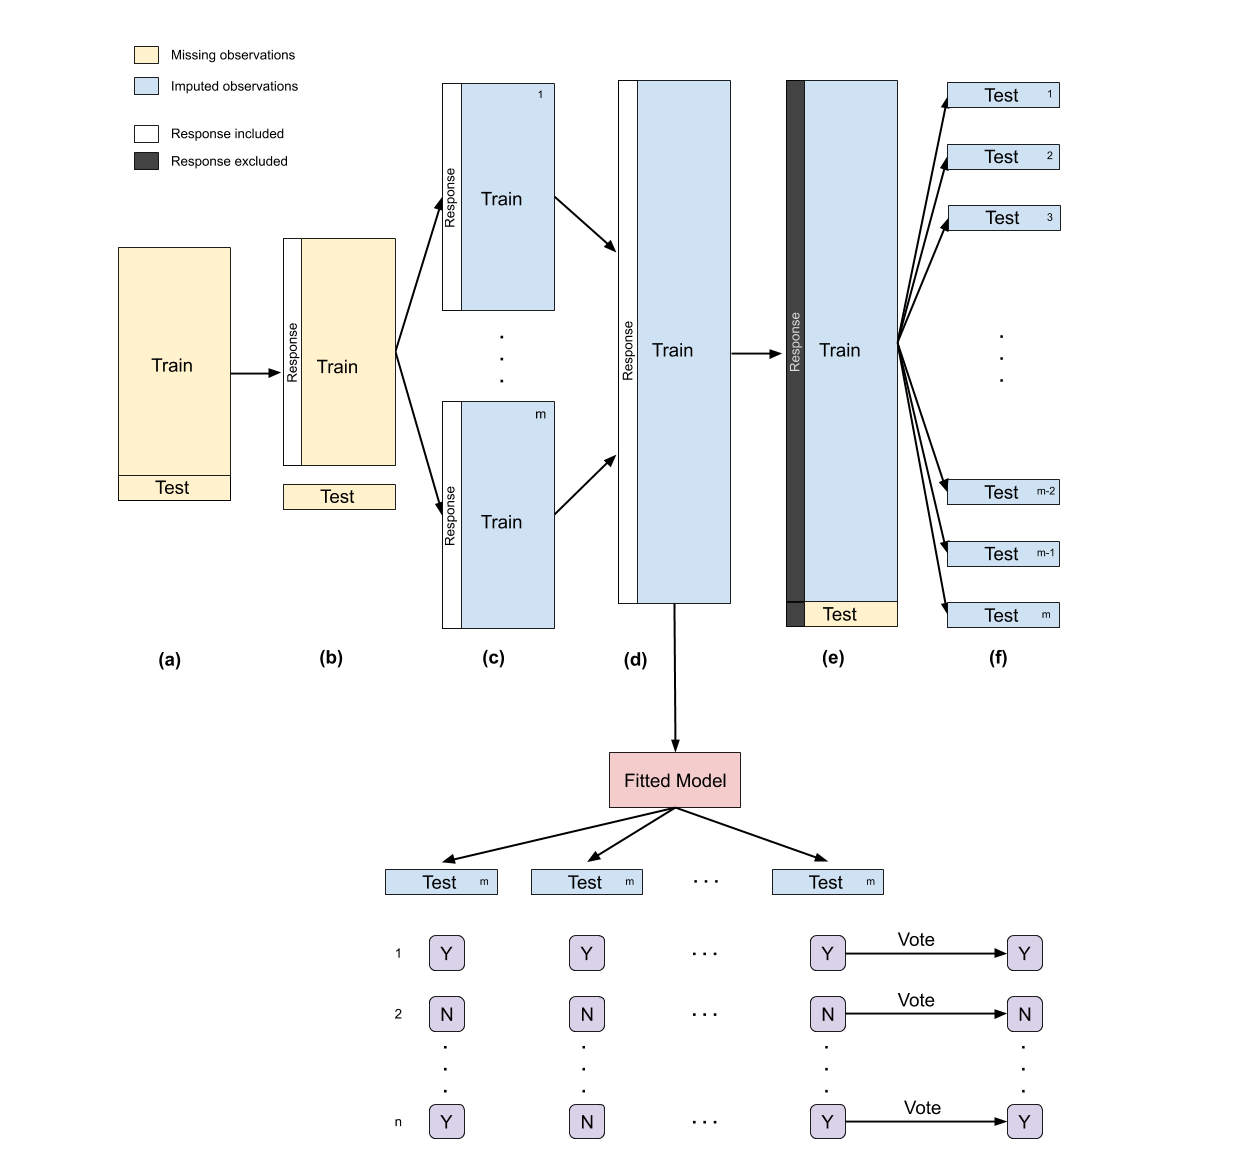
\includegraphics[width=1\linewidth]{images/ensemble-imputation} 

}

\caption{\label{fig:ensemble-imputation}Outline of Kth step in the ensemble algorithm used to combine MI in cross-validation.  (a) The Kth fold is taken as the test set (valid) and the remaining K-1 folds are taken as the training set. (b) Valid is separated from the analysis. (c) Train is imputed m times with the response included. (d) The m imputed datasets are 'stacked' to form one training set.  (e) Valid is concatenated with the imputed and 'stacked' training set.  (f) The test set is imputed m times using the imputed training set without the response included.  (g) A model is fitted to the imputed and 'stacked' training set.  (h) The fitted model makes predictions on each of the m valid sets.  (i) The m predictions are pooled by a majority vote.}\label{fig:unnamed-chunk-2}
\end{figure}

\newpage  

``Rubin's Rules'' (\protect\hyperlink{ref-rubin_inference_1976}{28})
provide a simple method for pooling parameters estimates from multiple
imputation for linear and generalized linear models but to the author's
knowledge, there has been insufficient work on estimating the required
number of imputations for estimating posterior probabilities in
classification problems. The classic advice for the choice of \(m\) is
between 3 and 5 for moderate amounts of missing information but it is
often beneficial to set \(m\) higher and create between 20-100
imputations (\protect\hyperlink{ref-van_buuren_flexible_2012}{1}).

There has been sufficient exploration into pooling of posterior
probabilities resulting from classification problems
(\protect\hyperlink{ref-kittler_combining_1996}{35},
\protect\hyperlink{ref-james_majority_1998}{36}), but there has been
little research into the pooling of predictions in classification
problems on multiply imputed datasets
(\protect\hyperlink{ref-belanche_handling_2014}{33}). Pooling multiple
predictions can be implemented using a variety of strategies, among
which majority vote is one of the simplest, and has been found to be
just as effective as more complicated schemes
(\protect\hyperlink{ref-lam_optimal_1995}{37}). Indeed, others have
pooled predictions from various classification methods by taking the
majority vote (\protect\hyperlink{ref-belanche_handling_2014}{33},
\protect\hyperlink{ref-james_majority_1998}{36}) and comparing
prediction performance.

This study involved four phases: (a) complete case analysis (CC) with
the variable \texttt{PreECMO\_Albumin} dropped from the analysis due to
46.44\% missingness, (b) mean imputation (SI1) on variables with missing
values, (c) imputation via the MICE algorithm implemented with PMM for
\(m=9\) imputed datasets (MI9), and (d) imputation via the MICE
algorithm implemented with PMM for \(m=99\) imputed datasets (MI99). In
each phase the data is first randomly stratified into 75\% training and
25\% test sets, with the test set held-out. Five classification models
are trained (Logit, KNN, LDA, QDA, RF) and tuned in 10-fold
cross-validation using the ensemble imputation described in Figure
\ref{fig:ensemble-imputation}. To determine the expected performance of
future predictions, one iteration of the ensemble imputation is
conducted for the full training set, the held-out test set, and the
tuned classification methods.

\subsection{Feature Selection}\label{feature-selection}

One of the goals of this analysis is to identify the variables most
useful for accurate prediction. There are various methods that can be
used for feature selection: stepwise selection, Recursive Feature
Elimination (RFE), LASSO regularization, and principle Component
Analysis (PCA). However, some of these methods are either highly
criticized, dependent on the classification method considered, or cannot
be integrated into the ensemble cross-validation approach used. Stepwise
selection, while very common, is only applicable to regression models
and it is often criticised
(\protect\hyperlink{ref-kemp_applied_2003}{38}); problems include
falsely narrow confidence intervals for effects and predicted values
(\protect\hyperlink{ref-altman_bootstrap_1989}{39}) and multiple
hypothesis testing inflating risks of capitalising on chance features of
the data (\protect\hyperlink{ref-altman_practical_1991}{40}), such as
noise covariates gaining entry into the model when the number of
candidate variables is large
(\protect\hyperlink{ref-derksen_backward_1992}{41}). RFE is an iterative
procedure analogous of backward feature selection. A new classifier is
trained on a subset of the features and the importance of the feature is
a measure of the change in performance. The training time scales
linearly with the number of classifiers to be trained
(\protect\hyperlink{ref-guyon_gene_2002}{42}). Both logistic regression
with LASSO regularization
(\protect\hyperlink{ref-tibshirani_regression_1996}{43}) and the
analogous Sparse Discriminant Analysis
(\protect\hyperlink{ref-clemmensen_sparse_2011}{44}) are embedded
feature selection methods that are dependent on the classification
method.

Principle Component Analysis (PCA)
(\protect\hyperlink{ref-f.r.s_liii._1901}{45}) is a feature extraction
method that is independent of the classification method. The training
set are orthogonally transformed into new uncorrelated variables called
principle components that are linear combinations of the original
variables. Feature extraction is accomplished by selecting the \(k\)
largest principle components that contain a chosen percent of the
variance in the original feature space.

PCA can also be used for feature selection by calculating the
contribution of each variable to the extracted features
(\protect\hyperlink{ref-song_feature_2010}{46}). Let \(C_i\) be the
contribution of a given variable on the principle component,
\(\text{V}_i\), and let \(\lambda_i\) be the eigenvalue of
\(\text{V}_i\), where \(\text{V}_{i} = \lambda_i \text{C}_i\). The
eigenvalues measure the amount of variation retained by each principle
component. The total contribution of a variable, \(\text{C}_j\), on
explaining the variations retained by \(k\) extracted features,
\(\text{V}_1, ..., \text{V}_k\), is

\[
\text{C}_j = \sum^k_{i=1} \vert \lambda_{ij} \text{C}_{ij} \vert = \sum^k_{p=1} \vert \text{V}_{ij} \vert   \tag{10}
\]

The \(\text{C}_j\) are sorted in descending order where \(\text{C}_1\)
contributes the most variation to the extracted principle components
among all the \(\text{C}_j\) for \(j=1,2,...p\), variables. Variables at
the beginning of the sorted list are considered more important for the
analysis than variables at the end. Here, any variable that contributes
more than the expected average contribution -- that is if all variables
contributed equally -- is selected as important for the analysis.

Variable selection via PCA is independent of the classification method
and allows important variables to be identified outside of the
classification analysis. The number of principle components retained,
\(k\), is based on the proportion of variance retained of the \(p\)
principle components, where the variance threshold is chosen to be 80\%.

\[
0.8 \leq \frac{\sum^k_{i=1} \lambda_i}{\sum^p_{j=1} \lambda_j}  \tag{11}
\] The number of principle components retained is based on the
proportion of variance. If the contribution of the \(p=30\) continuous
variables were uniform, the expected value would be \(1/\text{p} =\)
0.03. For a given component, an observation with a contribution larger
than this cutoff could be considered as important in contributing to the
component.

Variable selection is implemented using the \texttt{FactoMineR} package
(\protect\hyperlink{ref-husson_factominer:_2019}{47}).

\newpage

\section{Exploratory Data Analysis}\label{exploratory-data-analysis}

To get an idea of the distribution of the data, the following summary
statistics were obtained for the categorical variables in Table
\ref{tab:categorical-summaries} and for the continuous variables in
Figure \ref{fig:violin-standardised}.

\begin{table}[!h]

\caption{\label{tab:unnamed-chunk-3}\label{tab:categorical-summaries} Summary statistics for categorical variables.}
\centering
\fontsize{10}{12}\selectfont
\begin{tabular}{lccc}
\toprule
Variable & Level & n & \%\\
\midrule
 & N & 109 & 24.22\\

\multirow{-2}{*}{\raggedright\arraybackslash ECMO\_Survival} & Y & 341 & 75.78\\
\cmidrule{1-4}
 & m & 305 & 67.78\\

\multirow{-2}{*}{\raggedright\arraybackslash Gender} & w & 145 & 32.22\\
\cmidrule{1-4}
 & 1 & 66 & 14.67\\

 & 2 & 181 & 40.22\\

 & 3 & 31 & 6.89\\

 & 4 & 28 & 6.22\\

 & 5 & 71 & 15.78\\

 & 6 & 12 & 2.67\\

\multirow{-7}{*}{\raggedright\arraybackslash Indication} & 7 & 61 & 13.56\\
\bottomrule
\end{tabular}
\end{table}

Table \ref{tab:categorical-summaries} shows that the repsonse variable
\texttt{ECMO\_Survival} is imbalanced; of the 450 individuals, only
75.78\% in the study sample survived ECMO treatment (341 survived vs 109
did not survive). The variable \texttt{Gender} is also imbalanced with
only 67.78\% of the individuals in the study sample are male (305 male
vs 145 female). The distribution disease indication, \texttt{Indication}
shows a majority are of level 2 and levels 3, 4, and 6 relatively rare
occurances in this dataset.

Many of the standardised continuous variables in Figure
\ref{fig:violin-standardised} are highly skewed with a number of
outliers. This can affect the performance of discriminant analysis
classification methods that assume a distributional form for the data
(\protect\hyperlink{ref-hastie_elements_2009}{18}). The transformed
continuous variables are shown in Figure \ref{fig:violin-transformed}

The heatmap in Figure \ref{fig:heatmap-standardised} shows only a few
variables with moderate to strong correlation. Only a few variables,
\texttt{PreECMO\_NAdose} and \texttt{PreECMO\_Lactate}, are moderately
correlated with many other variable. Feature selection methods based on
the correlation matrix may not show strong feature importance for a
subset of the variables.

\subsection{Missing Data Exploration}\label{missing-data-exploration}

Before imputation, and indeed multiple imputation, it is important to
inspect the missingness patterns in the data and check assumptions.
Figure \ref{fig:missing-data} shows the missingness patterns in the
dataset, where a black bar represents a missing value. Many missing
values occur in observations with other missing values. The missing
values could be conditionally dependent on other variables, in which
case the data would be MAR. The missing values could also be due to some
unknown mechanism at the time of recording (\emph{i.e.} a failure of the
measurement device) that happens to effect multiple readings (the
biomarkers are measured from blood samples and measurements are likely
done in batches). In this case the data would be MCAR.

\begin{figure}[H]

{\centering \includegraphics[width=1\linewidth]{figure/graphics-unnamed-chunk-4-1} 

}

\caption{\label{fig:missing-data}Visual representation of missing observations in the ARDS dataset.}\label{fig:unnamed-chunk-4}
\end{figure}

From Figure \ref{fig:missing-data}, \texttt{PreECMO\_Albumin} is seen to
have 46.44\% missingness. To conserve more observations for the training
set, \texttt{PreECMO\_Albumin} is dropped from the complete case
analysis. Of the remaining variables only half contain missing values
with moderate to low missingness up to 6\%.

Table \ref{tab:missing-statistics} provides some measures about variable
dependence in the dataset. The first column shows the probability of
observed values for each variable. The following are coefficients that
give insight into how the variables are connected in terms of
missingness. \emph{Influx} is the ratio of the number of variables pairs
\((Y_j, ~Y_k)\) with \(Y_j\) missing and \(Y_k\) observed, divided by
the total number of observed data. For a variable that is entirely
missing, influx is 1, and 0 for if the variable is complete.
\emph{Outflux} is defined in the opposite manner, by dividing the number
of pairs \((Y_j, ~Y_k)\) with \(Y_j\) observed and \(Y_k\) missing, by
the total number of complete cells. For a completely observed variable,
outflux will have a value of 1 and 0 if completely missing. Outflux
gives an indication of how useful the variable will be for imputing
other variables in the dataset, while influx is an indicator for how
easily the variable can be imputed. Table \ref{tab:missing-statistics}
shows that all variables will be useful during impuation with the
exception of \texttt{PreECMO\_Albumin}. A high outflux variable might
turn out to be useless for the imputation procedure if it is unrelated
to the incomplete variables, while the usefulness of a highly predictive
variables is severely limited by a low outflux value
(\protect\hyperlink{ref-van_buuren_flexible_2012}{1}).

\newpage

\section{Results}\label{results}

\subsection{Prediction Performance}\label{prediction-performance}

This study involved four phases: (a) complete case analysis with the
variable \texttt{PreECMO\_Albumin} dropped from the analysis due to
46.44\% missingness, (b) mean imputation on variables with missing
values, (c) imputation via the MICE algorithm implemented with PMM for
\(m=9\) imputed datasets, and (d) imputation via the MICE algorithm
implemented with PMM for \(m=99\) imputed datasets.

The dataset was randomly stratified into 75\% training and 25\% test.
The five classification models were trained in 10-fold cross-validation
using the ensemble imputation approach. Table \ref{tab:cv-kappa} shows
the averaged Kappa from each analysis in 10-fold cross-validation. For
CC and SI1, LDA had the highest averaged Kappa, while logistic
regression had the highest averaged Kappa for MI9 and MI99.

\begin{table}[!h]

\caption{\label{tab:unnamed-chunk-5}\label{tab:cv-kappa} Averaged Cohen's Kappa for each model fitted in cross-validation.  The tuned parameters for KNN and RF on each imputation emthod are (a) K=5 and mtry=11(b) K=5 and mtry=11(c) K=5 and mtry=13 (d) K=13 and mtry=15, respectively.}
\centering
\fontsize{10}{12}\selectfont
\begin{tabular}{lrrrrr}
\toprule
  & Logit & LDA & QDA & KNN & RF\\
\midrule
CC & 0.139 & 0.205 & 0.038 & 0.053 & 0.035\\
SI1 & 0.191 & 0.220 & 0.040 & 0.136 & 0.085\\
MI9 & 0.179 & 0.124 & 0.106 & 0.088 & 0.136\\
MI99 & 0.185 & 0.158 & 0.037 & 0.127 & 0.177\\
\bottomrule
\end{tabular}
\end{table}

\emph{Validation on Test Set}

Using the parameters values learned in cross-validation (see Table
\ref{tab:cv-kappa}), models were fit on the full training set and
validated against the test set. Performance statistics are shown in
Table \ref{tab:metrics}. In complete case analysis, KNN with \(K=5\)
performed the best with \(\kappa=0.161\). For the mean-imputed data, RF
was the top performer with \(\kappa=0.197\). For both MI with \(m=9\)
(MI9) and \(m=99\) (MI99), logistic regression outperformed the other
classfication methods with \(\kappa=0.153\) and \(\kappa=0.274\),
respectively.

The highest overall accuracy was \(0.777\) using RF on the mean-imputed
dataset. However, the class-specific accuracies were \(0.965\) for
survival and \(0.185\) for non-survival. The best predictor of
non-survival was logistic regression on MI99.

\begin{table}[!h]

\caption{\label{tab:unnamed-chunk-6}\label{tab:metrics} Pooled performance results of trained models validated on test set.}
\centering
\fontsize{10}{12}\selectfont
\begin{tabular}{lccccc}
\toprule
 &  & Sensitivity & Specificity & Accuracy & Kappa\\
\midrule
 & Logit & 0.200 & 0.814 & 0.658 & 0.015\\

 & LDA & 0.200 & 0.847 & 0.684 & 0.054\\

 & QDA & 0.000 & 0.966 & 0.722 & -0.048\\

 & KNN & 0.300 & 0.847 & 0.709 & 0.161\\

\multirow{-5}{*}{\raggedright\arraybackslash CC} & RF & 0.050 & 0.966 & 0.734 & 0.022\\
\cmidrule{1-6}
 & Logit & 0.222 & 0.894 & 0.732 & 0.137\\

 & LDA & 0.148 & 0.894 & 0.714 & 0.051\\

 & QDA & 0.111 & 0.882 & 0.696 & -0.008\\

 & KNN & 0.222 & 0.824 & 0.679 & 0.050\\

\multirow{-5}{*}{\raggedright\arraybackslash SI1} & RF & 0.185 & 0.965 & 0.777 & 0.197\\
\cmidrule{1-6}
 & Logit & 0.222 & 0.906 & 0.741 & 0.153\\

 & LDA & 0.148 & 0.906 & 0.723 & 0.067\\

 & QDA & 0.111 & 0.882 & 0.696 & -0.008\\

 & KNN & 0.222 & 0.847 & 0.696 & 0.077\\

\multirow{-5}{*}{\raggedright\arraybackslash MI9} & RF & 0.148 & 0.941 & 0.750 & 0.116\\
\cmidrule{1-6}
 & Logit & 0.333 & 0.906 & 0.768 & 0.274\\

 & LDA & 0.185 & 0.906 & 0.732 & 0.111\\

 & QDA & 0.111 & 0.894 & 0.705 & 0.006\\

 & KNN & 0.185 & 0.882 & 0.714 & 0.080\\

\multirow{-5}{*}{\raggedright\arraybackslash MI99} & RF & 0.185 & 0.929 & 0.750 & 0.144\\
\bottomrule
\end{tabular}
\end{table}

\subsection{Feature Selection}\label{feature-selection-1}

From the PCA analysis, at least 16 principle components were needed to
explain 80\% of the variance in the imputed training data and at least
15 principle components for the complete case analysis. The red dashed
lines in Figure \ref{fig:feature-importance-pca} indicate the expected
average contribution of each variable to the selected principle
components if each variable contributed equally to each principle
component.

\begin{figure}[H]

{\centering 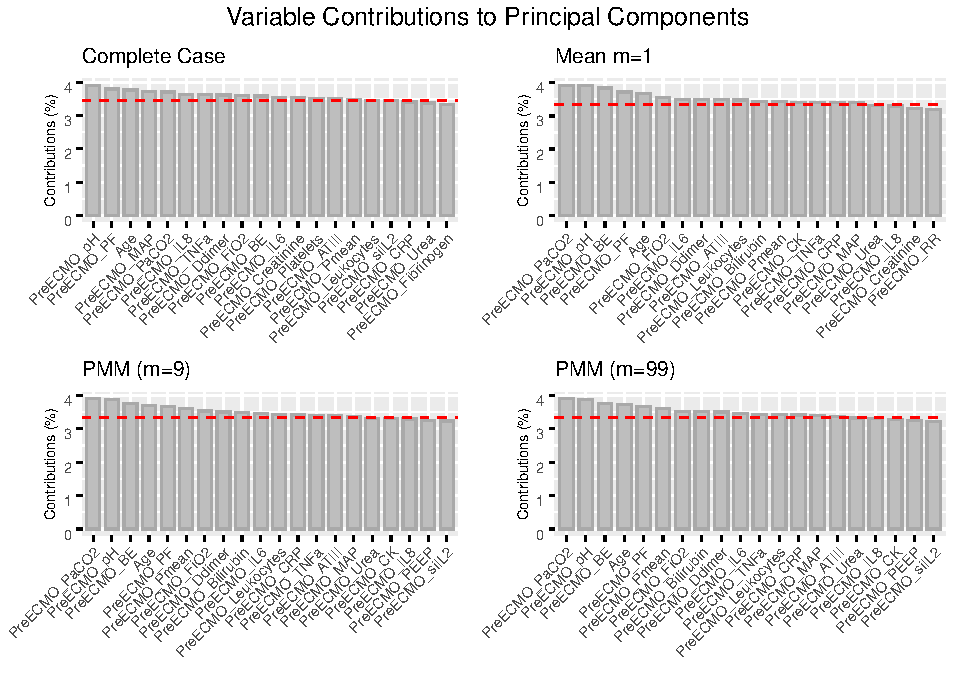
\includegraphics[width=1\linewidth]{figure/graphics-unnamed-chunk-7-1} 

}

\caption{\label{fig:feature-importance-pca}Contribution of variables to the principle components whose cumulative sum explains >80\% of the variation in the data.}\label{fig:unnamed-chunk-7}
\end{figure}

\newpage

\section{Discussion}\label{discussion}

Model performance on the imputed datasets were generally better than in
complete case analysis. Non-parametric methods, KNN and RF, performed
better on the complete case analysis and single mean imputation while
logistic regression performed better on the multiply imputed datasets.
All the methods in each analysis were able to predict survival with
\(>80\%\) accuracy. The ability to predict non-survival was the limiting
factor in the performance of a method. Non-survival was best predicted
by logistic regression in MI99 with a prediction accuracy of \(0.333\).

Logistic regression performed consistently well in predicting
non-survival and performed well for imputation methods except for
complete case analysis. LDA also performed rather consistently for each
imputed dataset. The consistent performance of LDA and logistic
regression is not surprising given that they are similar methods,
however logistic regression outperforms LDA in each analysis. LDA can
perform better than logistic regression when the covariates are normally
distributed (\protect\hyperlink{ref-efron_efficiency_1975}{48}), but LDA
is not robust to outliers
(\protect\hyperlink{ref-hastie_elements_2009}{18}) and Figure
\ref{fig:violin-standardised} shows a number of outliers in almost every
variable. Logistic regression is robust to outliers and makes less
assumptions than LDA (\protect\hyperlink{ref-hastie_elements_2009}{18})
allowing it to generalize better.

There were 136 less observations for complete case analysis than for the
other experiments. Performance metrics have moderate variance due to the
non-survival class in the test set only having 27 observations.
Predicting one or two more observations as non-survival can have
moderately large effects on Kappa. The relatively low number of
observations compounded by the imbalance in the response classes make
prediction difficult. Low predictive power of the variables make this
problem even more difficult.

A surprising result is that KNN performed the best on CC,
\(\kappa=0.161\) and also performed better than logistic regression on
MI9 (\(\kappa=0.153\)). RF performed poorly on CC (\(\kappa=0.022\)) but
was the best performer on SI1 (\(\kappa=0.197\)) and second best on MI9
and MI99 (\(\kappa=0.116\) and \(\kappa=0.144\)). The inverse
performance of KNN and RF may be surprising but Tang et al. show
(\protect\hyperlink{ref-tang_when_2018}{49}) that random forests can
perform poorly on datasets that work well for nearest-neighbor search
problems without sufficient subsampling, due to a lack of diversity. On
the imputed datasets KNN performed relatively poorly but similarly to
LDA. It should be noted that KNN consistently was able to predict
non-survival better than other methods, but at the cost of lower
accuracy in predicting survival. QDA consistently performed the worst,
no better than random chance based on the class likelihoods
(\(\kappa \approx 0\)), suggesting that the class distributions do not
support a quadratic decision boundary.

\(~\)\\
\emph{Feature Importance}

The selected variables via PCA were the same for SI1, MI9, and MI99 with
some variations in the order of importance. There were four selected
variables in CC that were not selected in the imputed datasets:
\texttt{PreECMO\_IL8}, \texttt{PreECMO\_Creatinine},
\texttt{PreECMO\_Platelets}, and \texttt{PreECMO\_SiL2}.

\subsection{Improvements}\label{improvements}

One way to increase predictive performance is to include more
observations in the analysis. Obtaining new data to include in the
analysis could prove expensive or difficult. Instead, some observations
from the test set could be retained for training the model in a nested
cross-validation approach. The analyses done in this paper would
constitute one iteration of the \(K_\text{o}\) outer cross-validation
iterations where a new test set is selected by stratified randomly
sampling, models are trained on the \(K_\text{o}-1\) via an inner
\(K_{i}\)-fold cross-validation. Since the data was originally split
into 25\% test and 75\% train, If \(K_\text{o}\) is chosen to be
\textgreater{}4, more observations can be retained in the training set.
If \(K_\text{o}=10\) were chosen, the prediction models would be trained
on 67 more observations. The outer cross-validtion would then give the
expected test prediction since it averages over different training sets
(\protect\hyperlink{ref-hastie_elements_2009}{18}). The drawback to
nested cross-validation is that the time complexity scales from
\(O(K_\text{i})\) to \(O(K_\text{o}K_\text{i})\). Indeed, the full time
complexity for \(m\) imputations and a grid search over \(p\) parameters
would then be \(O(pK_\text{o}K_\text{i}m)\).

The selected variables considered important in the survival prediction
of ARDS patients after ECMO treatment should be verified. A simple way
this can be done is by using only the variables shown as important in
Figure \ref{fig:feature-importance-pca} and conducting the ensemble
imputation. Realistically, this can only be done for CC and SI1. For MI9
and MI99, the important variables should be analysed for each imputed
dataset in the ensemble imputation algorithm. However, this adds another
layer of complexity and embedded variable selection methods would be a
more suitable option. Regularized logistic regression could be used to
select variables through use of the LASSO
(\protect\hyperlink{ref-tibshirani_regression_1996}{43}). LASSO methods
have also been developed for LDA and QDA: Sparse Discriminant Analysis
(\protect\hyperlink{ref-clemmensen_sparse_2011}{44}) and DALASS
(\protect\hyperlink{ref-trendafilov_dalass:_2007}{50}). Random forests
also naturally select important variables by accumulating the
improvement in the split-criterion over all the trees in the forest for
each variable (\protect\hyperlink{ref-hastie_elements_2009}{18}).

Weighted predictions can be obtained by pooling posterior probabilities
of the predictions using the arithmetic mean. Kittler et al.
(\protect\hyperlink{ref-kittler_combining_1996}{35}) show that
classifier combination strategies based on the sum (\emph{i.e}
arithmetic mean) are less sensitive to errors than strategies based on
the product (\emph{i.e} geometric mean) but perform just as well as a
majority vote. When combining predictions using the arithmetic mean,
more certain predictions (near 0 or 1) weight the prediction more than
uncertain predictions (near 0.5). Retaining posterior probabilities
would allow a choice in posterior probability cutoffs for predictions
and allow a performance analysis using ROC.

\subsection{Conclusion}\label{conclusion}

The CC has some distinctly different properties than the imputed
datasets; the best classification method was KNN, which performed
noteably worse in SI1, MI9, and MI99. The variables selected as
important for the predictions also differed in CC compared to the
imputed datasets. Given the curious results for CC, complete case
analysis may not be an appropriate method for handling the missing
values on the ARDS dataset. A more appropriate method would be mean
imputation or multiple imputation. ECMO treatment survival can be
predicted slightly better than random chance, \(\kappa=0.274\), using
logistic regression trained on MI99. Future expected prediction accuracy
for survival and non-survival of ECMO treatment are 0.906 and 0.333,
respectively. Variables deemed important for survival prediction are:
\texttt{PreECMO\_PaCO2}, \texttt{PreECMO\_pH}, \texttt{PreECMO\_Be},
\texttt{Age}, \texttt{PreECMO\_PF}, \texttt{PreECMO\_PMean},
\texttt{PreECMO\_FiO2}, \texttt{PreECMO\_Bilirubin},
\texttt{PreECMO\_Ddimer}, \texttt{PreECMO\_IL6}, \texttt{PreECMO\_TNFa},
\texttt{PreECMO\_Leukocytes}, \texttt{PreECMO\_CRP},
\texttt{PreECMO\_MAP}, and \texttt{PreECMO\_ATIII}.

\newpage

\section*{Appendices}\label{appendices}
\addcontentsline{toc}{section}{Appendices}

\subsection*{A. Additional Exploratory Data
Analysis}\label{a.-additional-exploratory-data-analysis}
\addcontentsline{toc}{subsection}{A. Additional Exploratory Data
Analysis}

\appendixA

\begin{figure}[H]

{\centering 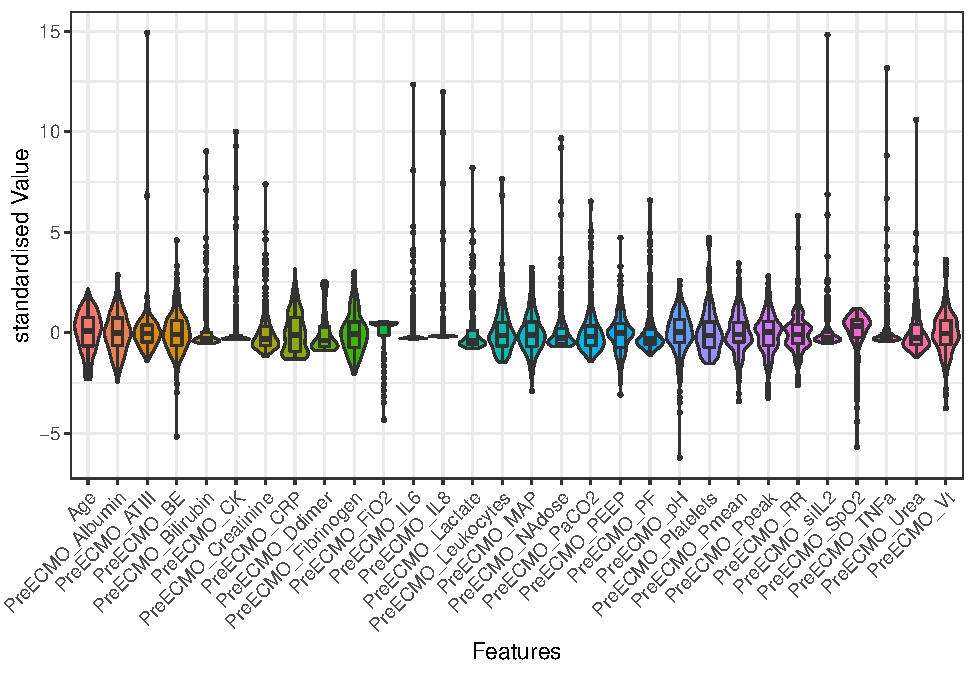
\includegraphics[width=0.75\linewidth]{figure/graphics-unnamed-chunk-8-1} 

}

\caption{\label{fig:violin-standardised}Violin plot of standardised continuous variables.}\label{fig:unnamed-chunk-8}
\end{figure}

\begin{figure}[H]

{\centering 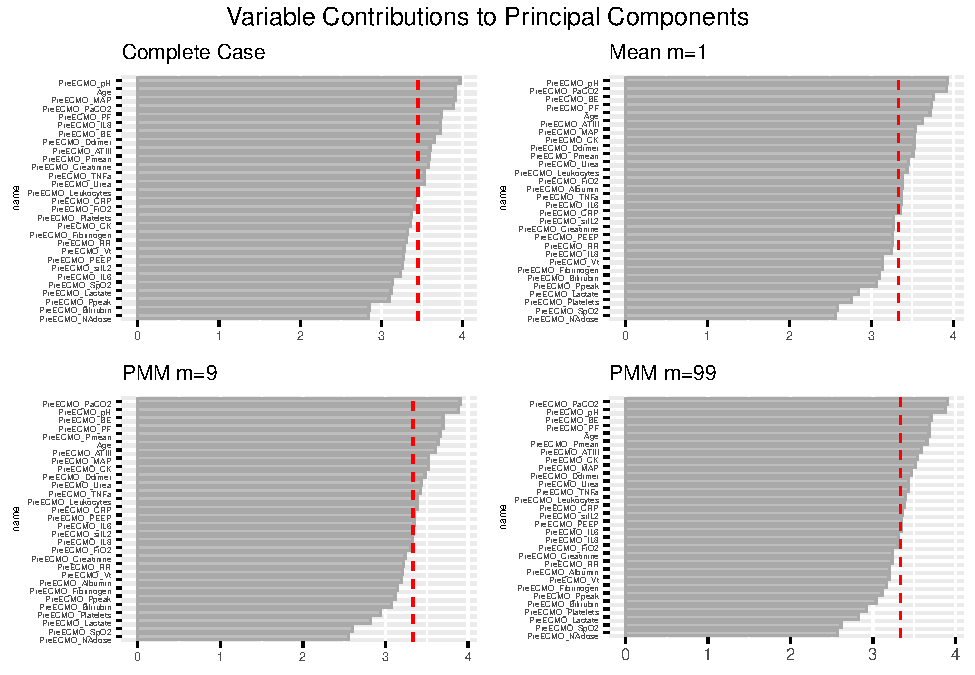
\includegraphics[width=0.75\linewidth]{figure/graphics-unnamed-chunk-9-1} 

}

\caption{\label{fig:violin-transformed}Violin plot of standardised and transformed continuous variables.}\label{fig:unnamed-chunk-9}
\end{figure}

\begin{figure}[H]

{\centering \includegraphics[width=1\linewidth]{figure/graphics-unnamed-chunk-10-1} 

}

\caption{\label{fig:heatmap-standardised}Heatmap of standardised and transformed variables.}\label{fig:unnamed-chunk-10}
\end{figure}

Table \ref{tab:missing-statistics} provides some measures about variable
dependence in the dataset. The first column shows the probability of
observed values for each variable. The following are coefficients that
give insight into how the variables are connected in terms of
missingness. \emph{Influx} is the ratio of the number of variables pairs
\((Y_j, ~Y_k)\) with \(Y_j\) missing and \(Y_k\) observed, divided by
the total number of observed data. For a variable that is entirely
missing, influx is 1, and 0 for if the variable is complete.
\emph{Outflux} is defined in the opposite manner, by dividing the number
of pairs \((Y_j, ~Y_k)\) with \(Y_j\) observed and \(Y_k\) missing, by
the total number of complete cells. For a completely observed variable,
outflux will have a value of 1 and 0 if completely missing. Outflux
gives an indication of how useful the variable will be for imputing
other variables in the dataset, while influx is an indicator for how
easily the variable can be imputed. Table \ref{tab:missing-statistics}
shows that all variables will be useful during impuation with the
exception of \texttt{PreECMO\_Albumin}. A high outflux variable might
turn out to be useless for the imputation procedure if it is unrelated
to the incomplete variables, while the usefulness of a highly predictive
variables is severely limited by a low outflux value
(\protect\hyperlink{ref-van_buuren_flexible_2012}{1}).

\begin{table}[!h]

\caption{\label{tab:unnamed-chunk-12}\label{tab:missing-statistics} Missing pattern statistics for variables in dataset.}
\centering
\fontsize{10}{12}\selectfont
\begin{tabular}{lrrr}
\toprule
  & Proportion & Influx & Outflux\\
\midrule
ECMO\_Survival & 1.00 & 0.00 & 1.00\\
Gender & 1.00 & 0.00 & 1.00\\
Indication & 1.00 & 0.00 & 1.00\\
Age & 1.00 & 0.00 & 1.00\\
PreECMO\_RR & 0.97 & 0.03 & 0.85\\
\addlinespace
PreECMO\_Vt & 0.97 & 0.03 & 0.85\\
PreECMO\_FiO2 & 1.00 & 0.00 & 1.00\\
PreECMO\_Ppeak & 0.97 & 0.03 & 0.85\\
PreECMO\_Pmean & 0.98 & 0.02 & 0.90\\
PreECMO\_PEEP & 0.97 & 0.03 & 0.85\\
\addlinespace
PreECMO\_PF & 1.00 & 0.00 & 1.00\\
PreECMO\_SpO2 & 1.00 & 0.00 & 1.00\\
PreECMO\_PaCO2 & 1.00 & 0.00 & 1.00\\
PreECMO\_pH & 1.00 & 0.00 & 1.00\\
PreECMO\_BE & 1.00 & 0.00 & 1.00\\
\addlinespace
PreECMO\_Lactate & 1.00 & 0.00 & 0.99\\
PreECMO\_NAdose & 1.00 & 0.00 & 1.00\\
PreECMO\_MAP & 0.99 & 0.01 & 0.97\\
PreECMO\_Creatinine & 1.00 & 0.00 & 1.00\\
PreECMO\_Urea & 0.98 & 0.02 & 0.94\\
\addlinespace
PreECMO\_CK & 0.95 & 0.05 & 0.87\\
PreECMO\_Bilirubin & 0.97 & 0.03 & 0.91\\
\textbf{PreECMO\_Albumin} & \textbf{0.54} & \textbf{0.46} & \textbf{0.26}\\
PreECMO\_CRP & 0.94 & 0.05 & 0.88\\
PreECMO\_Fibrinogen & 0.96 & 0.04 & 0.85\\
\addlinespace
PreECMO\_Ddimer & 0.95 & 0.04 & 0.86\\
PreECMO\_ATIII & 0.94 & 0.06 & 0.84\\
PreECMO\_Leukocytes & 1.00 & 0.00 & 0.99\\
PreECMO\_Platelets & 1.00 & 0.00 & 1.00\\
PreECMO\_TNFa & 0.98 & 0.02 & 0.93\\
\addlinespace
PreECMO\_IL6 & 1.00 & 0.00 & 1.00\\
PreECMO\_IL8 & 0.98 & 0.02 & 0.93\\
PreECMO\_siIL2 & 0.95 & 0.05 & 0.87\\
\bottomrule
\end{tabular}
\end{table}

\newpage

\subsection*{B. Algorithms}\label{b.-algorithms}
\addcontentsline{toc}{subsection}{B. Algorithms}

\appendixB

\subsubsection{Random Forests Algorithm}\label{random-forests-algorithm}

The random forests algorithm depicted is adapted from
(\protect\hyperlink{ref-hastie_elements_2009}{18}).

\begin{algorithm}[H]
\label{alg:random-forests-alg}
\caption{Random Forest Classifier}
\DontPrintSemicolon
\SetAlgoLined
\BlankLine

\begin{enumerate}
  \item For ($b=1$ to B):
    \begin{enumerate}
      \item Draw a bootstrap sample $\mathbf{Z*}$ of the size $N$ from the training data.
      \item Grow a random-forest tree $T_b$ to the bootstrapped data, by recursively repreating the following steps for each terminal node of the tree, until the minimum node size $n_{min}$ is reached.
      \begin{enumerate}
        \item Select $mtry$ variables at random from the $p$ covariates. 
        \item Pick the best covariate/split-point among the $mtry$. 
        \item Split the node into two daughter nodes. 
      \end{enumerate}
    \end{enumerate}
  \item Output the ensemble of trees $\{T_B\}^B_1$
\end{enumerate}
\BlankLine

Let $\hat{Y}_b(x)$ be the class prediction of the $b^{\text{th}}$ random-forest tree.  Then a new observation, $x$, is classified as:

$$\hat{Y}^B_{\text{rf}}(x) = \text{majority vote } \left\{ \hat{Y}_b(x) \right\}^B_1$$

\end{algorithm}

\subsubsection{MICE Algorithm}\label{mice-algorithm}

The MICE algorithm is adapted from
(\protect\hyperlink{ref-van_buuren_flexible_2012}{1}).

\begin{algorithm}[H]
\label{alg:mice-alg}
\caption{Multiple Imputation via Chained Equations}
\DontPrintSemicolon
\SetAlgoLined
\BlankLine

\begin{enumerate}
  \item Specify an imputation model $P(Y^{\text{mis}}_j \vert Y^{\text{obs}}_j, Y_{-j}, R)$ for variable $Y_j$ with $j=1,...,p$
  \item For each $j$, fill in starting imputation $Y^0_j$ by random draws from $Y^{\text{obs}}_j$
  \item Repeat for $t=1,...,T:$
  \item Repeat for $j=1,...,p:$
  \item Define $Y^t_{-j} = (Y^t_1,...,T^t_{j-1}, Y^{t-1}_{j+1},..., Y^{t-1}_p)$ as the currently complete data except $Y_j$ 
  \item Draw $\phi^t_j \sim P(\phi^t_j \vert Y^{\text{obs}}_j, Y^t_{-j}, R)$.
  \item Draw imputations from $Y^t_j \sim P(Y^{ \text{mis} }_j \vert Y^{ \text{obs} }_j, Y^t_{-j}, R, \phi^t_j)$.
  \item End repeat $j$.
  \item End repeat $t$.

\end{enumerate}
\BlankLine

\end{algorithm}

Using Equation 9 imputations are drawn under the normal linear model
using non-informative priors for each parameter. The required inputs
are:

\begin{itemize}
\tightlist
\item
  \(y_{\text{obs}}\), the \(n_1 \times 1\) vector of observed data in
  the target variable \(y\);
\item
  \(X_{\text{obs}}\), the \(n_1 \times q\) matrix of predictors of rows
  with observed data in \(y\);
\item
  \(X_{\text{mis}}\), the \(n_0 \times q\) matrix of predictors of rows
  with missing data in \(y\).
\end{itemize}

\begin{algorithm}[H]
\label{alg:pmm-alg}
\caption{Imputation of $y$ by predictive mean matching}
\DontPrintSemicolon
\SetAlgoLined
\BlankLine

\begin{enumerate}
  \item Calculate the cross-product matrix $S=X_{\text{obs}}'X_{\text{obs}}$.
  \item Calculate $V = (S + \text{diag}(S)\kappa)^{-1}$, with some small $\kappa$.
  \item Calculate regression weights $\hat{\beta} = V X_{\text{obs}}' y_{\text{obs}}$.
  \item Draw a random variable $\dot{g} \sim \chi^2_{\nu}$ with $\nu = n_1 - q$.
  \item Calculate $\dot{\sigma}^2 = (y_{\text{obs}} - X_{\text{obs}} \hat{\beta})' (y_{\text{obs}} - X_{\text{obs}} \hat{\beta}) / \hat{g}$.
  \item Draw $q$ independent $N(0,1)$ variate in vector $\dot{z}_1$.
  \item Calculate $V^{1/2}$ by Cholesky decomposition.
  \item Calculate $\dot{\beta} = \hat{\beta} + \dot{\sigma} \dot{z}_1 V^{1/2}$.
  \item Calculate $\dot{\eta}(i,j) = \vert X_{\text{obs},[i]} \hat{\beta} - X_{\text{mis},[j]} \dot{\beta} \vert$ with $i=1,...,n_1$ and $j=1,...,n_0$; 
  \item Construct $n_0$ sets $Z_j$, each containing $d$ candidate donors, from $Y_{\text{obs}}$ such that $\sum_d \dot{\eta}(i,j)$ is minimum for all $j=1,...,n_0$.  Break ties randomly;
  \item Draw one donor $i_j$ from $Z_j$ randomly for $j=1,...,n_0$
  \item Calculate imputations $\dot{y}_j - y_{i_j}$ for $j=1,...,n_0$.
\end{enumerate}

\BlankLine
\end{algorithm}

Where \(\kappa\) is a ridge parameter used to avoid problems with
singular matrices. The \emph{mice} package uses \(\kappa=1e-05\) as
default.

\newpage

\subsection*{C. Additional Missing Data
Diagnostics}\label{c.-additional-missing-data-diagnostics}
\addcontentsline{toc}{subsection}{C. Additional Missing Data
Diagnostics}

\appendixC

\subsubsection{Visual Insepction of
Imputations}\label{visual-insepction-of-imputations}

\begin{figure}[H]

{\centering 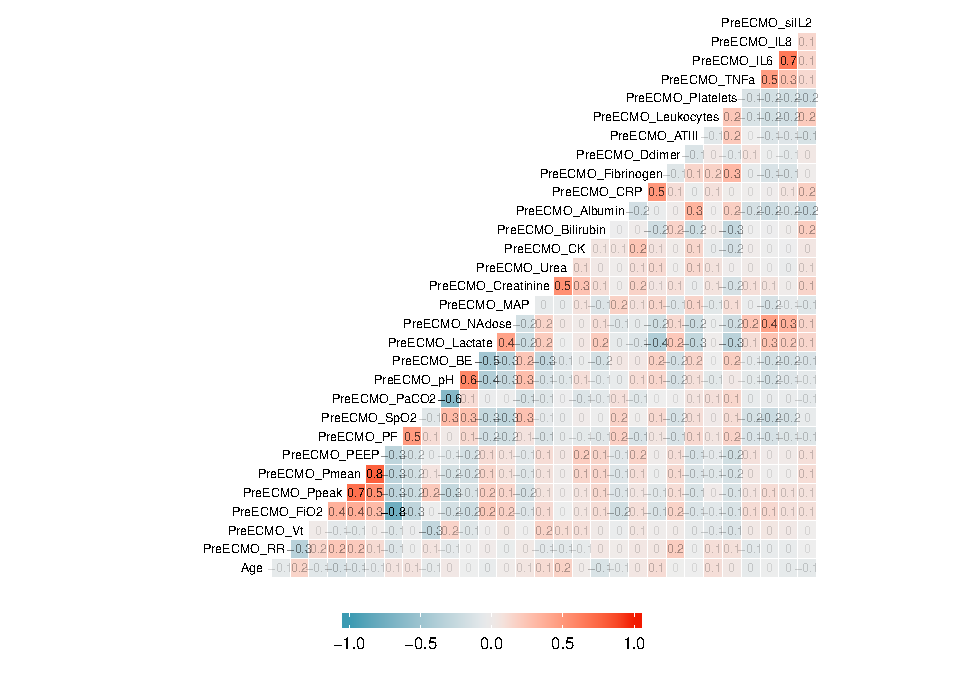
\includegraphics[width=0.75\linewidth]{figure/graphics-unnamed-chunk-14-1} 

}

\caption{\label{fig:xyplot-mean}Scatterplot of 9 mean imputed datasets.}\label{fig:unnamed-chunk-14}
\end{figure}

\begin{figure}[H]

{\centering 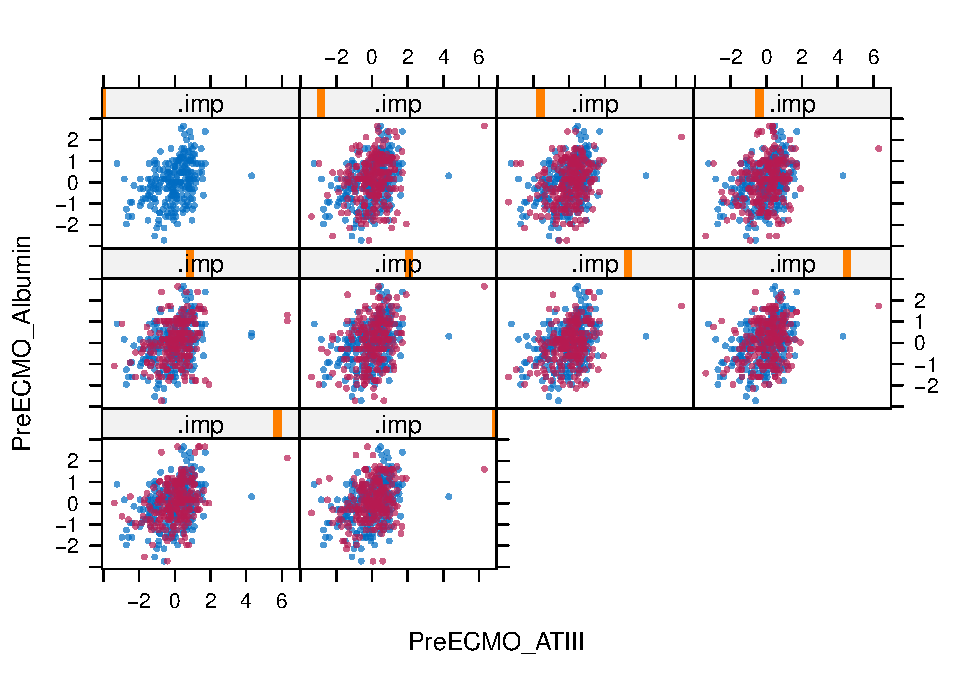
\includegraphics[width=0.75\linewidth]{figure/graphics-unnamed-chunk-15-1} 

}

\caption{\label{fig:xyplot-pmm}Scatterplot of the $m=9$ imputed datasets for MI9.  Can be extended to show similar results for MI99.}\label{fig:unnamed-chunk-15}
\end{figure}

\subsubsection{Convergence Monitoring}\label{convergence-monitoring}

\begin{figure}[H]

{\centering 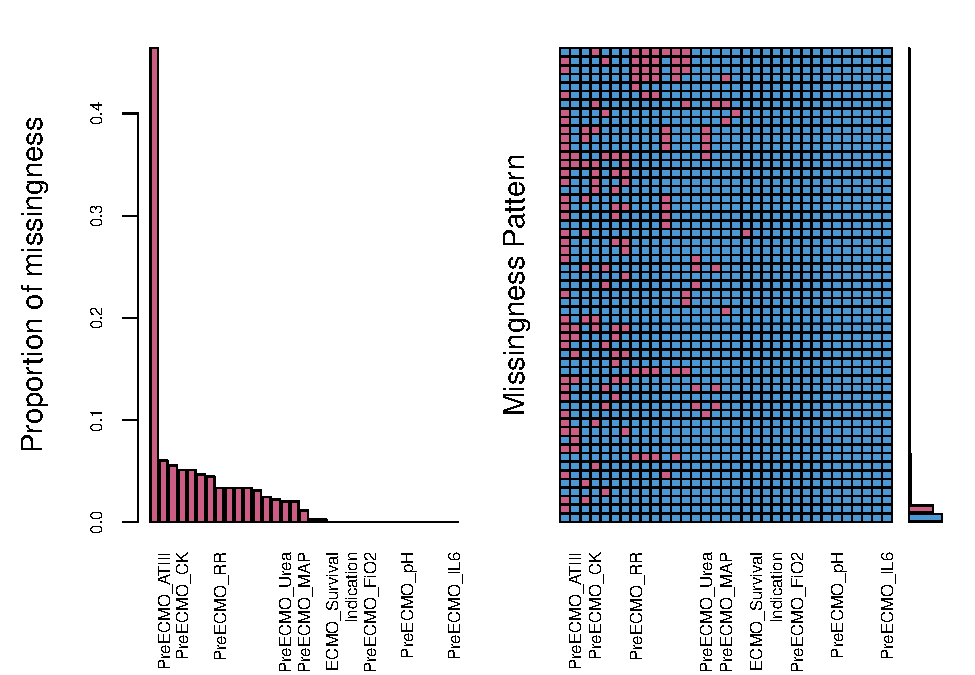
\includegraphics[width=0.75\linewidth]{figure/graphics-unnamed-chunk-16-1} 

}

\caption{\label{fig:converge-mean}Mean and standard deviation of the synthetic values plotted against iteration number for SI1.  The $m$ streams should intermingle with one another in convergence, without showing any definite trends.  Convergence occurs when the variance between different sequences is no larger than the variance within each individual sequence.}\label{fig:unnamed-chunk-161}
\end{figure}\begin{figure}[H]

{\centering 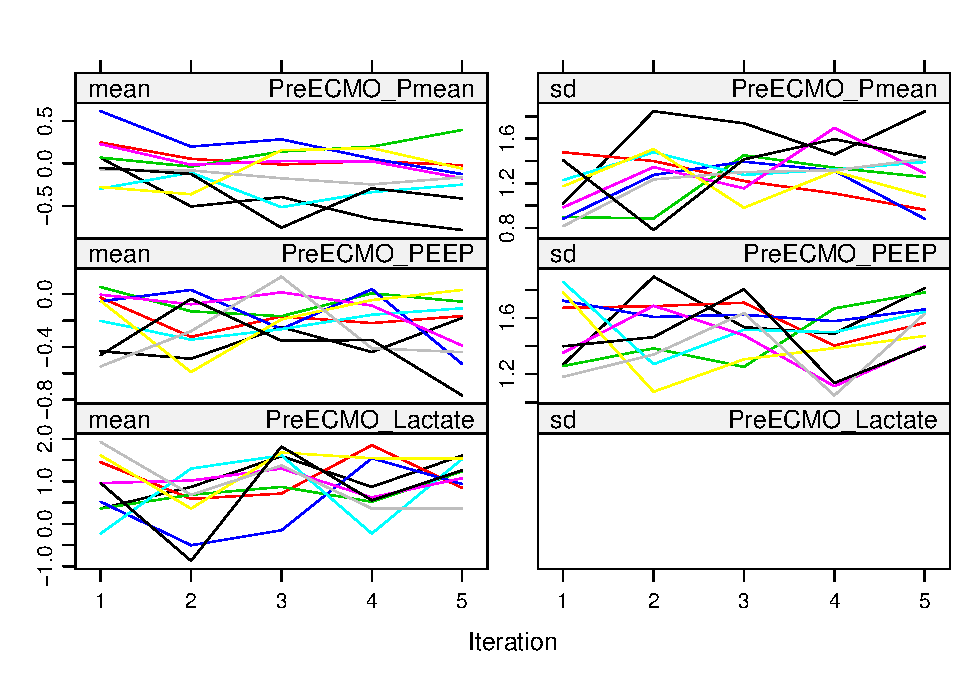
\includegraphics[width=0.75\linewidth]{figure/graphics-unnamed-chunk-16-2} 

}

\caption{\label{fig:converge-mean}Mean and standard deviation of the synthetic values plotted against iteration number for SI1.  The $m$ streams should intermingle with one another in convergence, without showing any definite trends.  Convergence occurs when the variance between different sequences is no larger than the variance within each individual sequence.}\label{fig:unnamed-chunk-162}
\end{figure}\begin{figure}[H]

{\centering 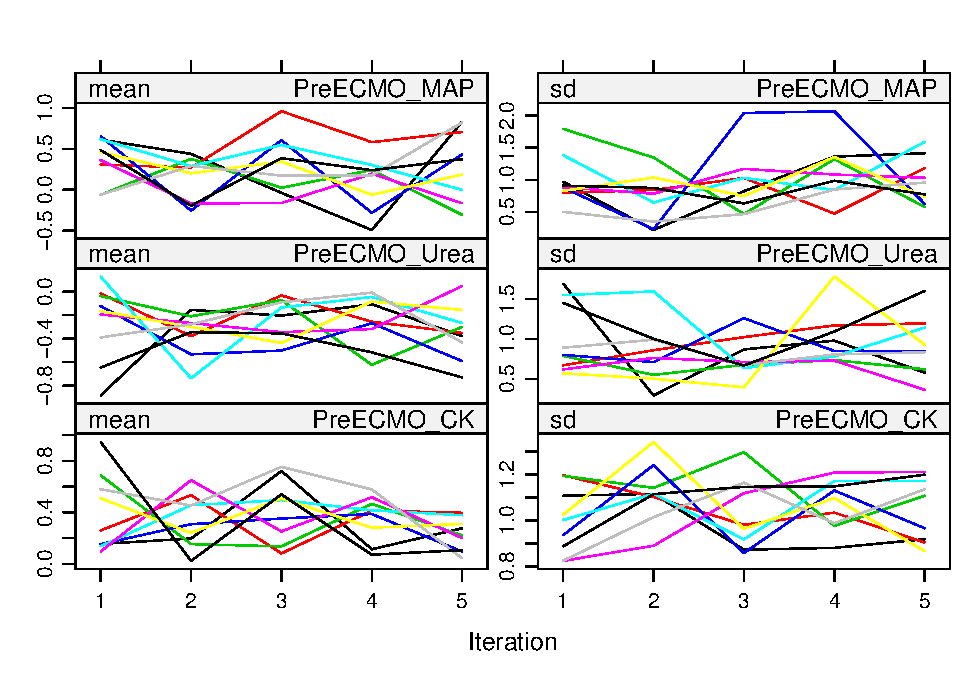
\includegraphics[width=0.75\linewidth]{figure/graphics-unnamed-chunk-16-3} 

}

\caption{\label{fig:converge-mean}Mean and standard deviation of the synthetic values plotted against iteration number for SI1.  The $m$ streams should intermingle with one another in convergence, without showing any definite trends.  Convergence occurs when the variance between different sequences is no larger than the variance within each individual sequence.}\label{fig:unnamed-chunk-163}
\end{figure}\begin{figure}[H]

{\centering 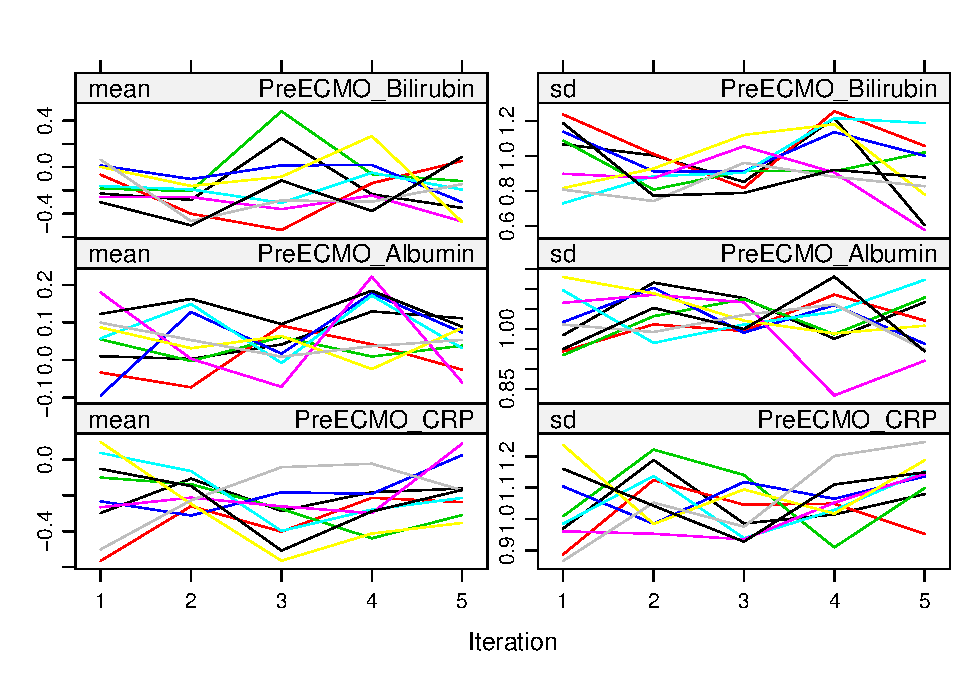
\includegraphics[width=0.75\linewidth]{figure/graphics-unnamed-chunk-16-4} 

}

\caption{\label{fig:converge-mean}Mean and standard deviation of the synthetic values plotted against iteration number for SI1.  The $m$ streams should intermingle with one another in convergence, without showing any definite trends.  Convergence occurs when the variance between different sequences is no larger than the variance within each individual sequence.}\label{fig:unnamed-chunk-164}
\end{figure}\begin{figure}[H]

{\centering 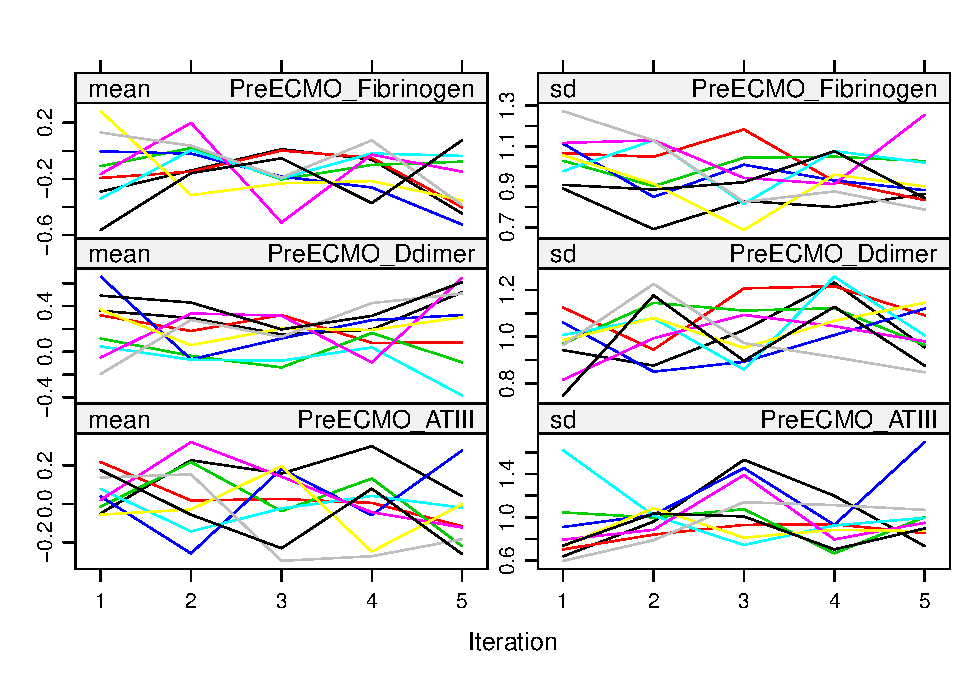
\includegraphics[width=0.75\linewidth]{figure/graphics-unnamed-chunk-16-5} 

}

\caption{\label{fig:converge-mean}Mean and standard deviation of the synthetic values plotted against iteration number for SI1.  The $m$ streams should intermingle with one another in convergence, without showing any definite trends.  Convergence occurs when the variance between different sequences is no larger than the variance within each individual sequence.}\label{fig:unnamed-chunk-165}
\end{figure}\begin{figure}[H]

{\centering 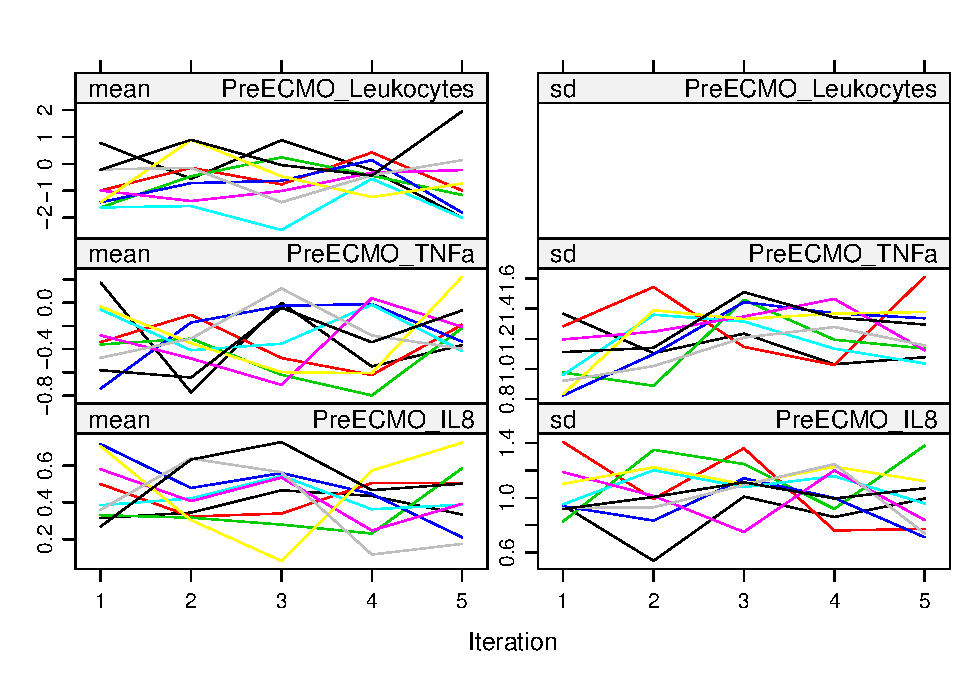
\includegraphics[width=0.75\linewidth]{figure/graphics-unnamed-chunk-16-6} 

}

\caption{\label{fig:converge-mean}Mean and standard deviation of the synthetic values plotted against iteration number for SI1.  The $m$ streams should intermingle with one another in convergence, without showing any definite trends.  Convergence occurs when the variance between different sequences is no larger than the variance within each individual sequence.}\label{fig:unnamed-chunk-166}
\end{figure}\begin{figure}[H]

{\centering 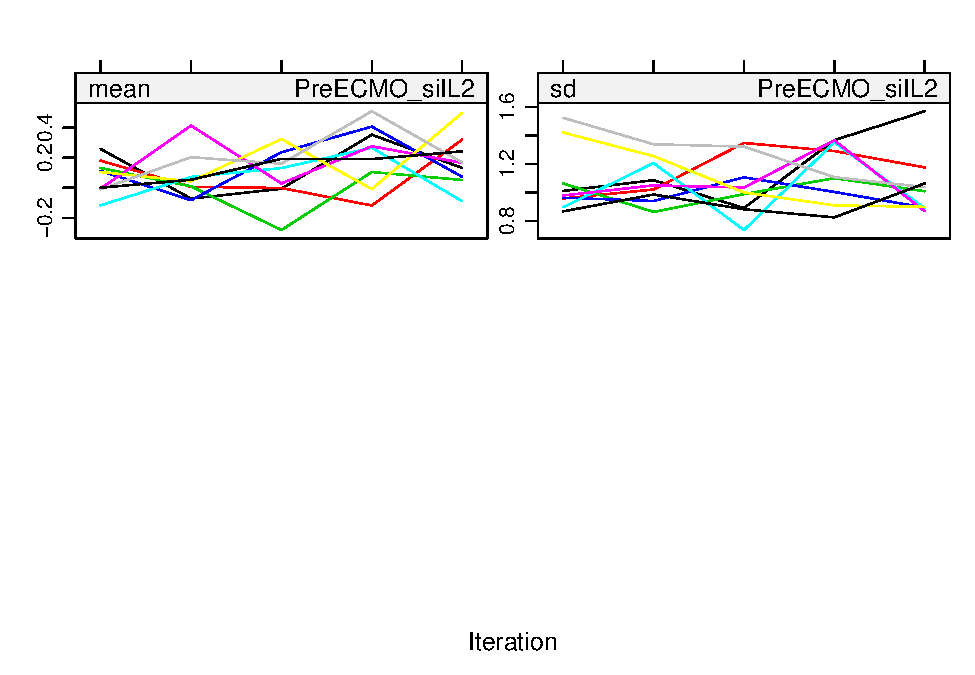
\includegraphics[width=0.75\linewidth]{figure/graphics-unnamed-chunk-16-7} 

}

\caption{\label{fig:converge-mean}Mean and standard deviation of the synthetic values plotted against iteration number for SI1.  The $m$ streams should intermingle with one another in convergence, without showing any definite trends.  Convergence occurs when the variance between different sequences is no larger than the variance within each individual sequence.}\label{fig:unnamed-chunk-167}
\end{figure}

\newpage

\subsection*{D. Code Structure}\label{d.-code-structure}
\addcontentsline{toc}{subsection}{D. Code Structure}

\appendixE

The code organization is described in Figure \ref{fig:r-code-chart}.
\texttt{libraries.R} contains all the libraries used in the analysis.
\texttt{functions.R} contains functions used in \texttt{training.R} and
\texttt{model-evaluation.R}. The ensemble cross-validation algorithm is
done in the \texttt{crossValidation()} function. The data is initially
cleaned and split into test and training sets in \texttt{preprocess.R}.
The cleaned datasets are saved to \texttt{processed-data.RData} for use
in \texttt{training.R} and in creating tables and figures in the thesis
rmarkdown. The training data is loaded into \texttt{training.R} where
each of the five classification methods are trained via ensemble
cross-validation. This is done for the four imputation methods: complete
case analysis, mean imputation, MICE using PMM for \(m=9\), and MICE
using PMM for \(m=99\) imputed datasets. The trained models for each
imputation method are saved into separate \texttt{trained-models.RData}.
The methods are then then fit to the full training set in
\texttt{model-evaluation.R} using the trained parameters found in
\texttt{training.R}. The final fitted models are evaluated on the test
set and the fitted models and performance metrics are saved to
\texttt{metrics.RData}.

\begin{figure}[H]

{\centering 
\includegraphics[width=1\linewidth]{images/r-code-chart} 

}

\caption{\label{fig:r-code-chart}Flowchart of code structure.}\label{fig:unnamed-chunk-17}
\end{figure}

\newpage

\section*{References}\label{references}
\addcontentsline{toc}{section}{References}

\hypertarget{refs}{}
\hypertarget{ref-van_buuren_flexible_2012}{}
1. Buuren S van (2012) \emph{Flexible Imputation of Missing Data}
(Chapman \& Hall, London). Second Edition.

\hypertarget{ref-schafer_missing_2002}{}
2. Schafer JL, Graham JW (2002) Missing data: Our view of the state of
the art. \emph{Psychological Methods} 7(2):147--177.

\hypertarget{ref-powney_review_2014}{}
3. Powney M, Williamson P, Kirkham J, Kolamunnage-Dona R (2014) A review
of the handling of missing longitudinal outcome data in clinical trials.
\emph{Trials} 15(1):237.

\hypertarget{ref-karahalios_review_2012}{}
4. Karahalios A, Baglietto L, Carlin JB, English DR, Simpson JA (2012) A
review of the reporting and handling of missing data in cohort studies
with repeated assessment of exposure measures. \emph{BMC medical
research methodology} 12:96--96.

\hypertarget{ref-wood_are_2004}{}
5. Wood AM, White IR, Thompson SG (2004) Are missing outcome data
adequately handled? A review of published randomized controlled trials
in major medical journals. \emph{Clinical Trials} 1(4):368--376.

\hypertarget{ref-mackinnon_use_2010}{}
6. Mackinnon A (2010) The use and reporting of multiple imputation in
medical research -- a review. \emph{Journal of Internal Medicine}
268(6):586--593.

\hypertarget{ref-hayati_rezvan_rise_2015}{}
7. Hayati Rezvan P, Lee KJ, Simpson JA (2015) The rise of multiple
imputation: A review of the reporting and implementation of the method
in medical research. \emph{BMC Medical Research Methodology} 15(1):30.

\hypertarget{ref-bellani_epidemiology_2016}{}
8. Bellani G, et al. (2016) Epidemiology, Patterns of Care, and
Mortality for Patients With Acute Respiratory Distress Syndrome in
Intensive Care Units in 50 CountriesTrends in Acute Respiratory Distress
Syndrome in 50 CountriesTrends in Acute Respiratory Distress Syndrome in
50 Countries. \emph{JAMA} 315(8):788--800.

\hypertarget{ref-rubenfeld_epidemiology_2007}{}
9. Rubenfeld GD, Herridge MS (2007) Epidemiology and Outcomes of Acute
Lung Injury. \emph{Chest} 131(2):554--562.

\hypertarget{ref-fan_acute_2018}{}
10. Fan E, Brodie D, Slutsky AS (2018) Acute Respiratory Distress
Syndrome: Advances in Diagnosis and TreatmentAcute Respiratory Distress
SyndromeAcute Respiratory Distress Syndrome. \emph{JAMA}
319(7):698--710.

\hypertarget{ref-paolone_extracorporeal_2017}{}
11. Paolone S (2017) Extracorporeal Membrane Oxygenation (ECMO) for Lung
Injury in Severe Acute Respiratory Distress Syndrome (ARDS): Review of
the Literature. \emph{Clinical Nursing Research} 26(6):747--762.

\hypertarget{ref-park_extracorporeal_2011}{}
12. Park PK, Napolitano LM, Bartlett RH (2011) Extracorporeal Membrane
Oxygenation in Adult Acute Respiratory Distress Syndrome. \emph{Critical
Care Clinics} 27(3):627--646.

\hypertarget{ref-wallace_ave_2010}{}
13. Wallace DJ, Milbrandt EB, Boujoukos A (2010) Ave, CESAR, morituri te
salutant! (Hail, CESAR, those who are about to die salute you!).
\emph{Critical Care} 14(2):308.

\hypertarget{ref-sahetya_survival_2018}{}
14. Sahetya SK, Brower RG, Stephens RS (2018) Survival of Patients With
Severe Acute Respiratory Distress Syndrome Treated Without
Extracorporeal Membrane Oxygenation. \emph{American Journal of Critical
Care} 27(3):220--227.

\hypertarget{ref-calfee_acute_2018}{}
15. Calfee CS (2018) Acute respiratory distress syndrome subphenotypes
and differential response to simvastatin: Secondary analysis of a
randomised controlled trial. \emph{The Lancet Respiratory Medicine}
6(9):691--698.

\hypertarget{ref-sinha_latent_2018}{}
16. Sinha P, et al. (2018) Latent class analysis of ARDS subphenotypes:
A secondary analysis of the statins for acutely injured lungs from
sepsis (SAILS) study. \emph{Intensive Care Medicine} 44(11):1859--1869.

\hypertarget{ref-yeo_new_2000}{}
17. Yeo I, Johnson RA (2000) A new family of power transformations to
improve normality or symmetry. \emph{Biometrika} 87(4):954--959.

\hypertarget{ref-hastie_elements_2009}{}
18. Hastie T, Tibshirani R, Friedman J (2009) \emph{The Elements of
Statistical Learning: Data Mining, Inference, and Prediction} (Springer)
Available at: \url{https://books.google.co.uk/books?id=eBSgoAEACAAJ}.

\hypertarget{ref-breiman_submodel_1992}{}
19. Breiman L, Spector P (1992) Submodel Selection and Evaluation in
Regression. The X-Random Case. \emph{International Statistical Review /
Revue Internationale de Statistique} 60(3):291--319.

\hypertarget{ref-kohavi_study_1995}{}
20. Kohavi R (1995) A Study of Cross-validation and Bootstrap for
Accuracy Estimation and Model Selection. \emph{Proceedings of the 14th
International Joint Conference on Artificial Intelligence - Volume 2},
IJCAI'95. (Morgan Kaufmann Publishers Inc., San Francisco, CA, USA), pp
1137--1143.

\hypertarget{ref-wing_caret:_2019}{}
21. Wing MKC from J, et al. (2019) Caret: Classification and Regression
Training. Available at: \url{https://CRAN.R-project.org/package=caret}
{[}Accessed August 29, 2019{]}.

\hypertarget{ref-fisher_use_1936}{}
22. FISHER RA (1936) THE USE OF MULTIPLE MEASUREMENTS IN TAXONOMIC
PROBLEMS. \emph{Annals of Eugenics} 7(2):179--188.

\hypertarget{ref-cover_geometrical_1965}{}
23. Cover TM (1965) Geometrical and Statistical Properties of Systems of
Linear Inequalities with Applications in Pattern Recognition. \emph{IEEE
Transactions on Electronic Computers} EC-14(3):326--334.

\hypertarget{ref-breiman_random_2001}{}
24. Breiman L (2001) Random Forests. \emph{Machine Learning}
45(1):5--32.

\hypertarget{ref-biau_random_2016}{}
25. Biau G, Scornet E (2016) A random forest guided tour. \emph{TEST}
25(2):197--227.

\hypertarget{ref-biau_analysis_2012}{}
26. Biau G (2012) Analysis of a Random Forests Model. \emph{J Mach Learn
Res} 13:1063--1095.

\hypertarget{ref-cohen_coefficient_1960}{}
27. Cohen J (1960) A Coefficient of Agreement for Nominal Scales.
\emph{Educational and Psychological Measurement} 20(1):37--46.

\hypertarget{ref-rubin_inference_1976}{}
28. RUBIN DB (1976) Inference and missing data. \emph{Biometrika}
63(3):581--592.

\hypertarget{ref-little_bayes_2014}{}
29. Little RJA, Rubin DB (2014) Bayes and Multiple Imputation.
\emph{Statistical Analysis with Missing Data} (John Wiley \& Sons, Ltd),
pp 200--220.

\hypertarget{ref-rubin_statistical_1986}{}
30. Rubin DB (1986) Statistical Matching Using File Concatenation With
Adjusted Weights and Multiple Imputations. \emph{Journal of Business \&
Economic Statistics} 4(1):87--94.

\hypertarget{ref-little_missing-data_1988}{}
31. Little RJA (1988) Missing-Data Adjustments in Large Surveys.
\emph{Journal of Business \& Economic Statistics} 6(3):287--296.

\hypertarget{ref-team_micemd:_2019}{}
32. team) VA(M, team) MR-R(E (2019) Micemd: Multiple Imputation by
Chained Equations with Multilevel Data. Available at:
\url{https://CRAN.R-project.org/package=micemd} {[}Accessed August 29,
2019{]}.

\hypertarget{ref-belanche_handling_2014}{}
33. Belanche LA, Kobayashi V, Aluja T (2014) Handling missing values in
kernel methods with application to microbiology data.
\emph{Neurocomputing} 141:110--116.

\hypertarget{ref-zavrakidis_combining_2017}{}
34. Zavrakidis I (2017) Combining Multiple Imputation with
cross-validation for calibration and assessment of Cox prognostic
survival models.

\hypertarget{ref-kittler_combining_1996}{}
35. Kittler J, Hater M, Duin RPW (1996) Combining classifiers.
\emph{Proceedings of 13th International Conference on Pattern
Recognition}, pp 897--901 vol.2.

\hypertarget{ref-james_majority_1998}{}
36. James G (1998) \emph{Majority Vote Classifiers: Theory and
Applications}.

\hypertarget{ref-lam_optimal_1995}{}
37. Lam L, Suen CY (1995) Optimal combinations of pattern classifiers.
\emph{Pattern Recognition Letters} 16(9):945--954.

\hypertarget{ref-kemp_applied_2003}{}
38. Kemp F (2003) Applied Multiple Regression/Correlation Analysis for
the Behavioral Sciences. \emph{Journal of the Royal Statistical Society:
Series D (The Statistician)} 52(4):691--691.

\hypertarget{ref-altman_bootstrap_1989}{}
39. Altman DG, Andersen PK (1989) Bootstrap investigation of the
stability of a cox regression model. \emph{Statistics in Medicine}
8(7):771--783.

\hypertarget{ref-altman_practical_1991}{}
40. Altman D (1991) \emph{Practical Statistics for Medical Research}
(Chapman \& Hall: London).

\hypertarget{ref-derksen_backward_1992}{}
41. Derksen S, Keselman HJ (1992) Backward, forward and stepwise
automated subset selection algorithms: Frequency of obtaining authentic
and noise variables. \emph{British Journal of Mathematical and
Statistical Psychology} 45(2):265--282.

\hypertarget{ref-guyon_gene_2002}{}
42. Guyon I, Weston J, Barnhill S, Vapnik V (2002) Gene Selection for
Cancer Classification using Support Vector Machines. \emph{Machine
Learning} 46(1):389--422.

\hypertarget{ref-tibshirani_regression_1996}{}
43. Tibshirani R (1996) Regression Shrinkage and Selection Via the
Lasso. \emph{Journal of the Royal Statistical Society: Series B
(Methodological)} 58(1):267--288.

\hypertarget{ref-clemmensen_sparse_2011}{}
44. Clemmensen L, Hastie T, Witten D, Ersbøll B (2011) Sparse
Discriminant Analysis. \emph{Technometrics} 53(4):406--413.

\hypertarget{ref-f.r.s_liii._1901}{}
45. F.R.S KP (1901) LIII. On lines and planes of closest fit to systems
of points in space. \emph{The London, Edinburgh, and Dublin
Philosophical Magazine and Journal of Science} 2(11):559--572.

\hypertarget{ref-song_feature_2010}{}
46. Song F, Guo Z, Mei D (2010) Feature Selection Using Principal
Component Analysis. \emph{2010 International Conference on System
Science, Engineering Design and Manufacturing Informatization}, pp
27--30.

\hypertarget{ref-husson_factominer:_2019}{}
47. Husson F, Josse J, Le S, Mazet J (2019) FactoMineR: Multivariate
Exploratory Data Analysis and Data Mining. Available at:
\url{https://CRAN.R-project.org/package=FactoMineR} {[}Accessed August
29, 2019{]}.

\hypertarget{ref-efron_efficiency_1975}{}
48. Efron B (1975) The Efficiency of Logistic Regression Compared to
Normal Discriminant Analysis. \emph{Journal of the American Statistical
Association} 70(352):892--898.

\hypertarget{ref-tang_when_2018}{}
49. Tang C, Garreau D, Luxburg U von (2018) When do random forests fail?

\hypertarget{ref-trendafilov_dalass:_2007}{}
50. Trendafilov NT, Jolliffe IT (2007) DALASS: Variable selection in
discriminant analysis via the LASSO. \emph{Computational Statistics \&
Data Analysis} 51(8):3718--3736.


\end{document}
